%%%%%%%%%%%%%%%%%%%%%%%%%%%%%%%%%%%%%%%%%
% INFORMATION (DO NOT CHANGE!)
%
% Doctoral Thesis (Chapter Based) University of Würzburg
% LaTeX Class
% Version 1.0 (03.2024)
%
% Author of Latex Template: 
% Martin Kuric 
% 
% Cover page is based on a template by the University of Würzburg
%
% This template is licensed under the GNU Public License v3.0
%%%%%%%%%%%%%%%%%%%%%%%%%%%%%%%%%%%%%%%%%

% ======================================================================
% == Preamble
% ======================================================================

\documentclass[12pt]{doctoral_thesis_uniwue} 

% :: Include only one part to work on for quicker compilation
% \includeonly{PARTS/2_INTRO_CANCER}
% \includeonly{PARTS/2_INTRO_CODING}
% \includeonly{PARTS/3_CHAPTER1}
% \includeonly{PARTS/3_CHAPTER2}
% \includeonly{PARTS/6_APPENDIX}


% ==============
% ==============
\begin{document}




% ======================================================================
% == Title Page + Submission + Project Institute 
% ======================================================================


% ======================================================================
% == Title Page 
% ======================================================================

% > Logo from:
% https://www.uni-wuerzburg.de/presse/service/bilder-und-grafik/corporate-design-vorlagen/logos/

\begin{titlepage}
    \begin{center}

        % == Sigil of the University of Würzburg ===============================
        \begin{figure}[H]
            \centering
            
\includegraphics[width=2.26in]{FIGS/0_neuSIEGEL.pdf}
        \end{figure}


        % == Title =============================================================
        \vspace{\vhalf}
        \rule{\textwidth}{0.4pt} \\ % thin horizontal line
        \vspace{7pt} % Make distances symmetrical

        Development and Semi-Automated Analysis of an \textit{in vitro} Dissemination Model \\
        for Myeloma Cells Interacting with Mesenchymal Stromal Cells
        \vspace{\vhalf}

        Entwicklung und semi-automatisierte Analyse eines \textit{in vitro} Modells \\
        für die Disseminierung von Myelomzellen in Interaktion mit mesenchymalen Stromazellen
        \rule{\textwidth}{0.4pt} % thin horizontal line



        % == University ========================================================
        \vspace{\vfull}
        {\large Doctoral Thesis for a Doctoral Degree } \\
        \vspace{\vhalf}
        \textit{at the} \\
        \vspace{\vhalf}
        \MakeUppercase{Graduate School of Life Sciences, \\
            Julius-Maximilians-Universität Würzburg, \\
            Section Biomedicine}


        % == Author ============================================================
        \vspace{\vhalf}
        \textit{submitted by} \\
        \vspace{\vhalf}
        {\Large \textbf{Martin Kuric}} \\
        \vspace{\vhalf}
        \textit{from} \\
        \vspace{\vhalf}
        \textbf{Bad Neustadt a.d. Saale}

        % == Date ==============================================================
        \vfill
        Würzburg, {\large 2024}

    \end{center}
\end{titlepage}
\thispagestyle{empty}   % Don't apply pagestyles to this page


\newpage

% == Blank Page ========================================================
\blankpage




% ======================================================================
% == Thesis Submission
% ======================================================================
\vspace*{\fill} % Shift it to bottom

\begin{adjustwidth}{+1cm}{+1cm} % Adjust the width of the page

    % == Date of Submission ================================================
    \noindent
    \begin{tabular}{l l}
        \textbf{Submitted on:} & \dotuline{\hspace{10cm}} \\
                               & {\small Office stamp}    \\
    \end{tabular}


    % == Promotionskomitee =================================================
    \vspace{\vdouble}
    {\noindent\large \textbf{Members of the \textit{Promotionskomitee}:}}

    \vspace{\vhalf}
    \begin{tabular}{l l}
        \textbf{Chairperson:}         & TODO: CHAIRPERSON                \\
        \textbf{Primary Supervisor:}  & Prof Dr. rer. nat. Regina Ebert  \\
        \textbf{Supervisor (Second):} & Prof Dr. med. Franziska Jundt    \\
        \textbf{Supervisor (Third):}  & Prof Dr. rer. nat. Torsten Blunk \\
    \end{tabular}


    % == Date of Defence, Certificate ======================================
    \vspace{\vdouble}
    \noindent
    \begin{tabular}{l l}
        \textbf{Date of Public Defense:}          & \dotuline{\hspace{6.45cm}} \\
                                                  &                            \\
        \textbf{Date of Receipt of Certificates:} & \dotuline{\hspace{6.45cm}} \\
    \end{tabular}

\end{adjustwidth}

\thispagestyle{empty} % > Don't apply pagestyles to this page


\newpage


% ======================================================================
% == Institue and Project Period
% ======================================================================
\vspace*{\fill} % > Shift it to bottom
\noindent
This work was conducted at the Department of Musculoskeletal Tissue
Regeneration (Bernhard-Heine-Centre for Locomotive Research), University
of Würzburg from 08.04.2018 to 31.03.2024 under the supervision of
Prof Dr.~rer.~nat.~Regina Ebert.

\thispagestyle{empty} % > Don't apply pagestyles to this page

\newpage


% ## Change page numbering to roman numerals
\setcounter{page}{1} % > Reset page counter to 1
\pagenumbering{roman}



% ======================================================================
% == Acknowledgements
% ======================================================================

\section*{Acknowledgements} % > Don't list in TOC
Lorem Ipsum dolor sit amet, consetetur sadipscing elitr, sed diam nonumy
eirmod tempor invidunt ut labore et dolore magna aliquyam erat, sed diam
voluptua. At vero eos et accusam et justo duo dolores et ea rebum. Stet
clita kasd gubergren, no sea takimata sanctus est Lorem ipsum dolor sit
amet. Lorem ipsum dolor sit amet, consetetur sadipscing elitr, sed diam
nonumy eirmod tempor invidunt ut labore et dolore magna aliquyam erat,
sed diam voluptua. At vero eos et accusam et justo duo dolores et ea
rebum. Stet clita kasd gubergren, no sea takimata sanctus est Lorem
ipsum

\newpage

% ======================================================================
% == Abstract
% ======================================================================

% > Include ABSTRACT.tex


% ======================================================================
% == Abstract
% ======================================================================


% == from paper ========================================================
% Abstract 1st paper (AACR):
% Multiple myeloma involves early dissemination of malignant plasma
% cells across the bone marrow; however, the initial steps of
% dissemination remain unclear. Human bone marrow-derived mesenchymal
% stromal cells (hMSCs) stimulate myeloma cell expansion (e.g., IL-6)
% and simultaneously retain myeloma cells via chemokines (e.g., CXCL12)
% and adhesion factors. Hence, we hypothesized that the imbalance
% between cell division and retention drives dissemination. 

% We present an in vitro model using primary hMSCs co-cultured with
% INA-6 myeloma cells. Time-lapse microscopy revealed proliferation and
% attachment/detachment dynamics. Separation techniques (V-well adhesion
% assay and well plate sandwich centrifugation) were established to
% isolate MSC-interacting myeloma subpopulations that were characterized
% by RNAseq, cell viability and apoptosis. Results were correlated with
% gene expression data (n=837) and survival of myeloma patients (n=536). 

% On dispersed hMSCs, INA-6 saturate hMSC-surface before proliferating
% into large homotypic aggregates, from which single cells detached
% completely. On confluent hMSCs, aggregates were replaced by strong
% heterotypic hMSC-INA-6 interactions, which modulated apoptosis
% time-dependently. Only INA-6 daughter cells (nMA-INA6) detached from
% hMSCs by cell division but sustained adherence to hMSC-adhering mother
% cells (MA-INA6).

% Isolated nMA-INA6 indicated hMSC-autonomy through superior viability
% after IL­6 withdrawal and upregulation of proliferation-related genes.
% MA-INA6 upregulated adhesion and retention factors (CXCL12), that,
% intriguingly, were highly expressed in myeloma samples from patients
% with longer overall and progression-free survival, but their
% expression decreased in relapsed myeloma samples. 

% Altogether, in vitro dissemination of INA-6 is driven by detaching
% daughter cells after a cycle of hMSC-(re)attachment and proliferation,
% involving adhesion factors that represent a bone marrow-retentive
% phenotype with potential clinical relevance.


% Summary 2nd paper (JOSS):
% plotastic addresses the challenges of transitioning from exploratory
% data analysis to hypothesis testing in Python’s data science ecosystem.
% Bridging the gap between seaborn and pingouin, this library offers a
% unified environment for plotting and statistical analysis. It simplifies
% the workflow with a user-friendly syntax and seamless integration with
% familiar seaborn parameters (y, x, hue, row, col). Inspired by seaborn’s
% consistency, plotastic utilizes a DataAnalysis object to intelligently
% pass parameters to pingouin statistical functions. The library
% systematically groups the data according to the needs of statistical
% tests and plots, conducts visualisation, analyses and supports extensive
% customization options. In essence, plotastic establishes a protocol for
% configuring statical analyses through plotting parameters. This approach
% streamlines the process, translating seaborn parameters into statistical
% terms, allowing researchers to focus on correct statistical testing and
% less about specific syntax and implementations.

% Statement of need 2nd paper (JOSS):
% Python’s data science ecosystem provides powerful tools for both
% visualization and statistical testing. However, the transition from
% exploratory data analysis to hypothesis testing can be cumbersome,
% requiring users to switch between libraries and adapt to different
% syntaxes.

% seaborn has become a popular choice for plotting in Python, offering an
% intuitive interface. Its statistical functionality focuses on
% descriptive plots and bootstrapped confidence intervals (Waskom, 2021).
% The library pingouin offers an extensive set of statistical tests, but
% it lacks integration with common plotting capabilities (Vallat, 2018).
% statannotations integrates statistical testing with plot annotations,
% but uses a complex interface and is limited to pairwise comparisons
% (Charlier et al., 2022).

% plotastic addresses this gap by offering a unified environment for
% plotting and statistical analysis. With an emphasis on user-friendly
% syntax and integration with familiar seaborn parameters, it simplifies
% the process for users already comfortable seaborn. The library ensures a
% smooth workflow, from data import to hypothesis testing and
% visualization


% == English ===========================================================
\renewcommand{\abstractname}{Summary}
\begin{abstract}
    Lorem Ipsum dolor sit amet, consetetur sadipscing elitr, sed diam nonumy
    eirmod tempor invidunt ut labore et dolore magna aliquyam erat, sed diam
    voluptua. At vero eos et accusam et justo duo dolores et ea rebum. Stet
    clita kasd gubergren, no sea takimata sanctus est Lorem ipsum dolor sit
    amet. Lorem ipsum dolor sit amet, consetetur sadipscing elitr, sed diam
    nonumy eirmod tempor invidunt ut labore et dolore magna aliquyam erat,
    sed diam voluptua. At vero eos et accusam et justo duo dolores et ea
    rebum. Stet clita kasd gubergren, no sea takimata sanctus est Lorem
    ipsum
\end{abstract}

% == German ============================================================
\renewcommand{\abstractname}{Zusammenfassung}
\begin{abstract}
    Lorem Ipsum dolor sit amet, consetetur sadipscing elitr, sed diam nonumy
    eirmod tempor invidunt ut labore et dolore magna aliquyam erat, sed diam
    voluptua. At vero eos et accusam et justo duo dolores et ea rebum. Stet
    clita kasd gubergren, no sea takimata sanctus est Lorem ipsum dolor sit
    amet. Lorem ipsum dolor sit amet, consetetur sadipscing elitr, sed diam
    nonumy eirmod tempor invidunt ut labore et dolore magna aliquyam erat,
    sed diam voluptua. At vero eos et accusam et justo duo dolores et ea
    rebum. Stet clita kasd gubergren, no sea takimata sanctus est Lorem
    ipsum bla
\end{abstract}

\newpage



% ======================================================================
% == Table of Contents
% ======================================================================

{\footnotesize \tableofcontents}

\newpage



% ======================================================================
% == Introduction
% ======================================================================
% > Change page numbering to arabic numerals
\pagenumbering{arabic}
\setcounter{page}{1} % > Reset page counter to 1

\unnsection{Introduction}
To provide a comprehensive background for the following chapters that focus on
the interaction of human mesenchymal stromal cells (hMSCs) with multiple myeloma
(MM) cells, this


% > Include 2_INTRO_CANCER.tex


% From paper 1 (AACR): Multiple myeloma arises from clonal expansion of
% malignant plasma cells in the bone marrow (BM). At diagnosis, myeloma cells
% have disseminated to multiple sites in the skeleton and, in some cases, to
% “virtually any tissue” (1,2). However, the mechanism through which myeloma
% cells initially disseminate remains unclear.

% Dissemination is a multistep process involving invasion, intravasation,
% intravascular arrest, extravasation, and colonization (3). To initiate
% dissemination, myeloma cells overcome adhesion, retention, and dependency on
% the BM microenvironment, which could involve the loss of adhesion factors such
% as CD138 (4,5). BM retention is mediated by multiple factors: First,
% chemokines (CXCL12 and CXCL8) produced by mesenchymal stromal cells (MSCs),
% which attract plasma cells and prime their cytoskeleton and integrins for
% adhesion (6,7). Second, myeloma cells must overcome the anchorage and physical
% boundaries of the extracellular matrix (ECM), consisting of e.g. fibronectin,
% collagens, and proteoglycans such as decorin (8–11). Simultaneously, ECM
% provides signals inducing myeloma cell cycle arrest or progression the cell
% cycle (8,11). ECM is also prone to degradation, which is common in several
% osteotropic cancers, and is the cause of osteolytic bone disease. This is
% driven by a ‘vicious cycle’ that maximizes bone destruction by extracting
% growth factors (EGF and TGF-β) that are stored in calcified tissues (12).
% Third, direct contact with MSCs physically anchors myeloma cells to the BM
% (3,13). Fourth, to disseminate to distant sites, myeloma cells require, at
% least partially, independence from essential growth and survival signals
% provided by MSCs in the form of soluble factors or cell adhesion signaling
% (5,14,15). For example, the VLA4 (Myeloma)–VCAM1 (MSC)-interface activates
% NF-κB in both myeloma and MSCs, inducing IL-6 expression in MSCs. The
% independence from MSCs is then acquired through autocrine survival signaling
% (16,17). In short, anchorage of myeloma cells to MSCs or ECM is a
% ‘double-edged sword’: adhesion counteracts dissemination, but also presents
% signaling cues for growth, survival, and drug resistance (18).

% To address this ambiguity, we developed an in vitro co-culture system modeling
% diverse adhesion modalities to study dissemination, growth, and survival of
% myeloma cells and hMSCs. Co-cultures of hMSCs and the myeloma cell line INA-6
% replicated tight interactions and aggregate growth, akin to "microtumors" in
% Ghobrial’s metastasis concept (19). We characterized the growth conformations
% of hMSCs and INA­6 as homotypic aggregation vs. heterotypic hMSC adherence and
% their effects on myeloma cell survival. We tracked INA­6 detachments from
% aggregates and hMSCs, thereby identifying a potential "disseminated"
% subpopulation lacking strong adhesion. We developed innovative techniques
% (V-well adhesion assay and well plate sandwich centrifugation) to separate
% weakly and strongly adherent subpopulations for the subsequent analysis of
% differential gene expression and cell survival. Notably, our strategy resolves
% the differences in gene expression and growth behavior between cells of one
% cell population in "direct" contact with MSCs. In contrast, previous methods
% differentiated between "direct" and "indirect" cell-cell contact using
% transwell inserts (20). To evaluate whether genes mediating adhesion and
% growth characteristics of INA-6 were associated with patient survival, we
% analyzed publicly available datasets (21,22).


% ======================================================================
% ======================================================================
\unnsubsection{Human Mesenchymal Stem/Stromal Cells}
Explaining what a mesenchymal stromal cell (MSC) is, is not such an easy task as
one might expect. MSCs are derived from multiple\ MSCs different sources, serve
a wide array of functions and are always isolated as a heterogenous group of
cells. This makes it particularly challenging to find a consensus on their exact
definition, nomenclature, exact function and \textit{in vivo} differentiation
potential. Therefore, the most effective approach to describe hMSCs is to
present their historical context.

hMSCs first gained popularity as a stem cell. Stem cells lay the foundation of
multicellular organisms. Embryonic stem cells orchestrate the growth and
patterning during embryonic development, while adult stem cells are responsible
for regeneration during adulthood. The classical definition of a stem cell is
that of a relatively undifferentiated cell that divides asymmetrically,
producing another stem cell and a differentiated
cell~\cite{cooperCellMolecularApproach2000, shenghuiMechanismsStemCell2009}.
Because of their significance in biology and regenerative medicine, stem cells
have become a prominent subject in modern research. Especially human mesenchymal
stromal cells (hMSCs) have proven to be a promising candidate in this
context~\cite{ullahHumanMesenchymalStem2015}.

Mesenchyme first appears in embryonic development during gastrulation. There,
cells that are committed to a mesodermal fate, lose their cell junctions and
exit the epithelial layer in order to migrate freely. This process is called
epithelial-mesenchymal transition
\cite{tamFormationMesodermalTissues1987,nowotschinCellularDynamicsEarly2010}.
Hence, the term mesenchyme describes non-epithelial embryonic tissue
differentiating into mesodermal lineages such as bone, muscles and blood.
Interestingly, it was shown nearly twenty years earlier that cells within adult
bone marrow seemed to have mesenchymal properties as they were able to
differentiate into bone tissue
\cite{friedensteinOsteogenesisTransplantsBone1966,friedensteinOsteogenicPrecursorCells1971,biancoMesenchymalStemCells2014}.
This was the origin of the ``mesengenic process''-hypothesis: This concept
states that mesenchymal stem cells serve as progenitors for multiple mesodermal
tissues (bone, cartilage, muscle, marrow stroma, tendon, fat, dermis and
connective tissue) during both adulthood and embryonic
development~\cite{caplanMesenchymalStemCells1991,caplanMesengenicProcess1994}.
The mesenchymal nature of these cells (termed bone marrow stromal cells: BMSCs)
was confirmed later when they were shown to differentiate into adipocytic (fat)
and chondrocytic (cartilage)
lineages~\cite{pittengerMultilineagePotentialAdult1999}. Since then, the term
``mesenchymal stem cell'' (MSC) has grown popular as an adult multipotent
precursor to a couple of mesodermal tissues. hMSCs derived from bone marrow
(hMSCs) were shown to differentiate into osteocytes, chondrocytes, adipocytes
and cardiomyocytes
\cite{gronthosSTRO1FractionAdult1994,muruganandanAdipocyteDifferentiationBone2009,xuMesenchymalStemCells2004}
Most impressively, these cells also exhibited
ectodermal and endodermal differentiation potential, as they produced
neuronal cells, pancreatic cells and hepatocytes
\cite{barzilayLentiviralDeliveryLMX1a2009,wilkinsHumanBoneMarrowderived2009,gabrInsulinproducingCellsAdult2013,stockHumanBoneMarrow2014}.

Furthermore, cultures with MSC properties can be established from ``virtually
every post-natal organs and tissues'', and not just bone
marrow~\cite{dasilvameirellesMesenchymalStemCells2006}. However, it has to be
noted that hMSCs can differ greatly in their transcription profile and
\textit{in vivo} differentiation potential depending on which tissue they
originated from
\cite{jansenFunctionalDifferencesMesenchymal2010,sacchettiNoIdenticalMesenchymal2016}.

Since ``hMSCs' are a heterogenous group of cells, they were defined by their
\textit{in vitro} characteristics. A minimal set of criteria are the following
\cite{dominiciMinimalCriteriaDefining2006}: First, hMSCs must be plastic
adherent. Second, they must express or lack a set of specific surface antigens
(positive for CD73, CD90, CD105; negative for CD45, CD34, CD11b, CD19). Third,
hMSCs must differentiate to osteoblasts, adipocytes and chondroblasts \textit{in
    vitro}. Together, hMSCs exhibit diverse differentiation potentials and can be
isolated from multiple sources of the body. This offers great opportunity for
regenerative medicine, if the particular hMSC-subtype is properly characterized.


% ======================================================================
% ======================================================================
\unnsubsection{Multiple Myeloma}
Multiple myeloma arises from clonal expansion of malignant plasma cells in the
bone marrow (BM). At diagnosis, myeloma cells have disseminated to multiple
sites in the skeleton and, in some cases, to virtually any
tissue~\cite{rajkumarMultipleMyelomaCurrent2020,
    bladeExtramedullaryDiseaseMultiple2022}.


% ======================================================================
% ======================================================================
\unnsubsection{Myeloma-hMSC Interactions}
Since plasma cells can not survive outside the bone marrow, MM cells also
require survival signals for growth and disease progression. These signals are
produced by the bone marrow microenvironment, including ECM, MSCs and
ACs~\cite{kiblerAdhesiveInteractionsHuman1998,
    garcia-ortizRoleTumorMicroenvironment2021}.


% ======================================================================
% ======================================================================
\unnsubsection{Myeloma Bone Disease}
Bone is a two-phase system in which the mineral phase provides the stiffness and
the collagen fibers provide the ductility and ability to absorb
energy~\cite{viguet-carrinRoleCollagenBone2006}. On a molecular level, bone
tissue is composed of extracellular matrix (ECM) proteins that are calcified by
hydroxyapatite crystals. This ECM consists mostly of collagen type I, but also
components with major regulatory activity, such as fibronectin and proteoglycans
that are essential for healthy bone
physiology~\cite{alcorta-sevillanoDecipheringRelevanceBone2020}. Bone tissue is
actively remodeled by bone-forming osteoblasts and bone-degrading osteoclasts.
Osteoblasts are derived from mesenchymal stromal cells (MSCs) that reside in the
bone marrow~\cite{friedensteinOsteogenesisTransplantsBone1966,
    pittengerMultilineagePotentialAdult1999}. MSCs also give rise to adipocytes
(ACs) to form Bone Marrow Adipose Tissue (BMAT), which can account for up to
70\% of bone marrow volume~\cite{fazeliMarrowFatBone2013}.

MM indirectly degrades bone tissue by stimulating osteoclasts and inhibiting
osteoblast differentiation, which leads to MM-related bone disease
(MBD)~\cite{glaveyProteomicCharacterizationHuman2017}. MBD is present in 80\% of
patients at diagnosis and is characterized by osteolytic lesions, osteopenia and
pathological fractures~\cite{terposPathogenesisBoneDisease2018}.


% ======================================================================
% ======================================================================
\unnsubsection{Dissemination of Myeloma Cells}
dissemination is still widely unclear
- multistep process
- invasion, intravasation, intravascular arrest, extravasation,
colonization
- overcome adhesion, retention, and dependency on the BM
microenvironment
- loss of adhesion factors such as CD138

% > New Page to separate biological part from the technical part 

% > Include 2_INTRO_CODING.tex


% ======================================================================
\unnsubsection{Code-Automation as a Standard in Modern Biosciences}
\
Beschreibe die Situation.
- Big Data in Biosciences
- what is big data, examples
- Define citable challenges:
- reproducibility crisis
- lack of tools

% - Semi big data
% - What is that: At the edge of managability
% - Tools to handle semi-big data are lacking:
% Either manual analysis or big data tools
% - Author defines semi-automation



In recent years, the biosciences have evolved dramatically, with a marked
increase in the volume and complexity of data generated
~\cite{yangScalabilityValidationBig2017,ekmekciIntroductionProgrammingBioscientists2016}.
This transformation necessitates robust software tools, many of which require
coding skills to use effectively. Here we summarize standard tools used by
biosciences today and show their reliance on coding. The author argues that the
role of a modern independent researcher is now intertwined with coding skills
similar to a role of ``precision medicine
bioninformatician''~\cite{gomez-lopezPrecisionMedicineNeeds2019}.

Statistical analysis in biosciences has traditionally been reliant on
user-friendly tools like Excel and GraphPad Prism. While Excel by itself is
recognized as limited for complex data analysis
\cite{tanavaleeLimitationsUsingMicrosoft2016a, incertiYouStillUsing2019a},
GraphPad Prism offers more advanced statistical models .

However, increasingly demands more sophisticated
approaches as data sets grow in size and complexity.

R and Python scripts offer more efficient and
versatile solutions, enabling complex analyses with a few lines of code
\cite{rcoreteamLanguageEnvironmentStatistical2018,vallatPingouinStatisticsPython2018}.

Recognizing this trend, Microsoft has integrated a Python interpreter into Excel to
computations more accessible within a widely used platform \cite{AnnouncingPythonExcel2023}.

% A potential use-case for coding is statistical analysis. Most users rely on tools
% like Prism.
% However, Prism becomes impractical with large and complex datasets,
% as manual re-analysis is time-consuming. In contrast, scripts in R or Python
% allow for a single click to re-analyze the data. Recognizing this trend,
% Microsoft has recently implemented a Python interpreter into Excel, allowing
% execution of python code within cells. R, in particular, offers more advanced
% statistical models than Prism or Excel, which has led to R's widespread
% adoption.

Next-generation sequencing, such as bulk RNAseq, has become affordable, allowing
for larger sample sets during a single PhD project. This technology offers
advanced tools that are most efficiently used through scripting in R or Python.
In the absence of a dedicated statistician, researchers are compelled to learn
coding.

In gene ontology, tools such as Metascape facilitate the integration of vast
datasets and outputs multiple useful data visualizations. Metascape also
provides multiple excel sheets, containing all results, sometimes in a nested
format, which provides even further information that's adaptable for specific
hypotheses, but given the sheer amount of data, is impractical to analyze
manually.

since Metascape
returns large Excel sheets with complex nested information, a researcher without
coding skills requires manual work to adapt the results to specific research
hypotheses.

its true potential is unlocked only when researchers can
manipulate and analyze these data through scripting.

Modern gene ontology tools like Metascape offer powerful graphical user
interfaces. However, their effectiveness is only possible through standardizing
multiple large datasets.

The output from Metascape, large Excel sheets with
complex nested information, is more efficiently analyzed through scripting,
which is often necessary to adapt metascape results to specific research
hypotheses.



Image analysis is another area where coding skills are essential. ImageJ/FIJI, a
standard tool in the field, requires scripting for batch processing of multiple
images and automating multiple processing steps into a pipeline. While macros
can be recorded, understanding the underlying code is necessary for
troubleshooting and adapting the macro to new datasets.

In the field of protein structural biology, Pymol is a standard tool that also
has a Python command interface.

Similarly, artificial intelligence (AI), a
game-changer in biomedicine, primarily uses Python due to its extensive
libraries for machine learning and scientific computing. Python is also a
standard for integrative biomedicine simulations.

Finally, databases and repositories are essential for storing, retrieving, and
sharing data. Researchers need to understand common file formats to adhere to
standards that ensure re-usability and interoperability. Scripting helps
automate the process of formatting data for submission to these databases.

In conclusion, the integration of coding in bioscience research is not just a
trend but a necessity. As the field continues to evolve, the demarcation between
biologists and computational scientists blurs, underscoring the importance of
coding skills for the next generation of researchers. The ability to code is
fast becoming an indispensable asset, as integral to bioscience as traditional
laboratory skills.



%%%%%%%%%%%%%%%

% In the last decades, biosciences have made significant progress in generating
% vast amounts of data in shorter time spans
% ~\cite{yangScalabilityValidationBig2017}. Here, it is argued that research reliant
% on software more than ever. More so, the author of the thesis highly doubts that
% every modern researcher will be confronted with executing at least some lines of
% code during their career, or maybe even collect multiple commands in a
% self-written script.


% - The question is, can a modern PhD student fulfill their role as an independent
% researcher without coding skills? This is highly questionable, given that
% standard tools in the biosciences require a code interface:


% - Statistics? No. Requires Prism, but Prism becomes unpractical with large and
% complex datasets, since manual re-analysis has to be repeated manually, while
% scripts would allow for a single click to re-analyze the data. Hence, R or
% Python have become a standard, with R offering more advanced statistical models
% than Prism or Excel. Excel has recognized this development and
% introduced Python support

% - Next generation sequencing? Rnaseq has become cheap (bulk RNAseq), allowing for growing
% samplesets during one PhD project, while gaining in remarkable
% precision, even at single-cell level. It offers advanced tools, that are only
% used efficiently scripting in R or Python. If
% there's no dedicated statistician, researchers have no choice but to learn
% coding

% - Gene ontology: Modern tools like metascape offer a surprisingly powerful
% graphical user interface. Still this achievement is only possible through
% standardizing multiple large datasets. Also the output of metascape are large
% excel sheets with highly complex nested information. These that are unpractical
% to analyze manually by excel and are more efficiently analyzed through scripting
% to adapt to specific needs of research hypotheses.

% - Image analysis? ImageJ/FIJI is standard. However, there are bugs. Also,
% scripting is required for both batch processing of multiple images and also
% automating multiple processing steps into a pipeline. Of course, macros can be
% recorded, yet an understanding of the underlying code is required to
% troubleshoot and adapt the macro to new datasets.

% - Protein structurual biologists? Pymol is standard and also has a python
% command interface

% - Artificial intelligence (AI) has been a game changer in the field of
% biomedicine. The early development of AI itself was driven by radiology, where
% it was designed to detect pathologies in medical images. Today, Python is a
% standard because of its extensive libraries for machine learning and scientific
% computing.


% - Integrative biomedicine simulations? Python is a standard

% - In general, coding skills help improve a researchers general understanding of
% every software he uses. This is because the researcher can understand the
% underlying algorithms and assumptions of the software. Complex proprietary
% software to use state-of-the-art equipment (Zen, Imaris, FlowJo, etc.) are often
% black boxes. The researcher will be confronted with issues and has to make
% constant decisions if the error is on his side, or on the software side in order
% to think of feasable troubleshooting strategies. This is only possible if the
% researcher has a good understanding of the software. A basic understanding of
% code also opens the door to open-source software, allowing for state-of-the-art
% analysis techniques that are not available in proprietary software, but their
% installation and usage is often overestimated by researchers without coding
% skills, while coding skills allow for adaptations of this software to the
% specific needs of the researcher.

% - Furthermore, databases and repositories are essential for storing, retrieving,
% and sharing data. In order to adhere to standards that ensure re-usability and
% interoparability, researchers need to have an understanding of common file
% formats. Scripting also helps to automate the process of formatting data for
% submitting to these databases.

% Together, it remains highly questionable, if future scientists will be able to
% perform their role as independent researchers without minimum coding skills.
% In conclusion, the increasing role of software in biomedicine underscores the
% importance of computational skills for modern researchers. As the field
% continues to evolve, the ability to work with software will become even more
% critical.

%%%%%%%%%%%%%%%%



% Modern methods in molecular biology, biochemistry, and biomedicine, such as
% next-generation sequencing, mass spectrometry, and high-throughput screening,
% generate large volumes of data that require sophisticated software tools for
% analysis. For instance, bioinformatics software is essential for analyzing
% genomic and proteomic data, while image analysis software is routinely used in
% microscopy.


% Moreover, the rise of systems biology and integrative biomedicine, which aim to
% understand biological systems as a whole, has led to the development of complex
% computational models and simulation software. These tools are used to integrate
% and analyze diverse data types, from molecular to physiological data, and to
% predict the behavior of biological systems.


% In addition, software plays a crucial role in the management and sharing of
% biomedical data. Databases and data repositories are essential for storing,
% retrieving, and sharing data, while data standards and ontologies, which are
% often implemented as software libraries, are used to ensure that data is
% interoperable and reusable.


% Given this landscape, it is clear that researchers in the biosciences are
% confronted with complex software on a daily basis. Therefore, there is a growing
% need for researchers to acquire computational skills.

% Learning a programming
% language like Python can greatly benefit researchers by enabling them to
% automate tasks, analyze data more efficiently, and develop their own tools. This
% not only increases productivity but also fosters reproducibility and open
% science.


% In conclusion, the increasing role of software in biomedicine underscores the
% importance of computational skills for modern researchers. As the field
% continues to evolve, the ability to work with software will become even more
% critical.





% ======================================================================
\unnsubsection{How Code Quality Improves Scientific Reproducibility}
A main reason to write software is to define re-usable instructions for task
automation~\cite{narztReusabilityConceptProcess1998}. However, the complexity of
the code makes it prone to errors and can prevent usage by persons other than
the author himself. This is a problem for the general scientific community, as
the software is often the only way to reproduce the results of a
study~\cite{sandveTenSimpleRules2013}. Hence, modern journals aim to enforce
standards to software development, including software written and used by
biological researchers~\cite{smithJournalOpenSource2018}. Here, we provide a
brief overview of the standards utilized by \texttt{plotastic} that to ensure
its reliability and reproducibility by the scientific community~\cite{pengReproducibleResearchComputational2011}.

Modern software development is a long-term commitment of maintaining and
improving code after initial release~\cite{boswellArtReadableCode2011}. Hence,
it is good practice to write the software such that it is scalable, maintainable
and usable. Scalability or, to be precise, structural scalability means that the
software can easily be expanded with new features without major modifications to
its architecture \cite{bondiCharacteristicsScalabilityTheir2000}. This is
achieved by writing the software in a modular fashion, where each module is
responsible for a single function. Maintainability means that the software can
easily be fixed from bugs and adapted to new requirements
\cite{kazmanMaintainability2020}. This is achieved by writing the code in a
clear and readable manner, and by writing tests that ensure that the code works
as expected~\cite{boswellArtReadableCode2011}. Usability is hard to
define~\cite{brookeSUSQuickDirty1996}, yet one can consider a software as usable
if the commands have intuitive names and if the software's manual, termed
``documentation'', is up-to-date and easy to understand for new users with
minimal coding experience. A software package that has not received an update
for a long time (approx. one year) could be considered abandoned. Abandoned
software is unlikely to be fully functional, since it relies on other software
(dependencies) that has changed in functionality or introduce bugs that were not
expected by the developers of all dependencies. Together, software that's
scalable, maintainable and usable requires continuous changes to its codebase.
There are best practices that standardize the continuous change of the codebase,
including version control, continuous integration (often referred to as CI), and
software testing.

Version control is a system that records changes to the codebase line by line,
allowing the documentation of the history of the codebase, including who made
which changes and when. This is required to isolate new and experimental
features into newer versions and away from the stable version that's known to
work. The most popular version control system is Git, which is considered the
industry standard for software development~\cite{chaconGitBook2024}. Git can use
GitHub.com as a platform to store and host codebases in the form of software
repositories. GitHub's most famous feature is called ``pull request''. A pull
request is a request from anyone registered on GitHub to include their changes
to the codebase (as in ``please pull this into your main code''). One could see
pull requests as the identifying feature of the open source community, since it
exposes the codebase to potentially thousands of independent developers,
reaching a workforce that is impossible to achieve with closed source models
used by paid software companies.

Continuous integration (CI) is a software development practice in which
developers integrate code changes into a shared repository several times a
day~\cite{duvall2007continuous}. Each integration triggers the test suite,
aiming to detect errors as soon as possible. The test suite includes building
the software, setting up an environment for the software to run and then
executing the programmed tests, ensuring that the software runs as a whole.
Continuous integration is often used together with software branches. Branches
are independent copies of the codebase that are meant to be merged back into the
original code once the changes are finished. Since branches accumulate multiple
changes over time, this can lead to minor incompatibilities between the branches
of all developers (integration conflicts), which is something that CI helps to
prevent.

Continuous integration especially relies on a thorough software testing suite.
Software testing is the practice of writing code that checks if the codebase
works as expected~\cite{10.5555/2161638}. The main type of software testing is
unit testing, which tests the smallest units of the codebase (functions and
classes) in isolation (\autoref{lst:unit_test}).

\def\mycaption{ Example of an arbitrary python function and its respective unit
    test function. The first function simply returns the number 5. The second
    function tests if the first function indeed returns the number 5. The test
    function is named with the prefix ``\texttt{test\_}'' and is placed in a
    file that ends with the suffix ``\texttt{\_test.py}''. The test function is
    executed by the testing framework \texttt{pytest}. Note that code after
    ``\texttt{\#}'' is considered a comment and won't be executed.}
\begin{lstlisting}[
    language=Python, 
    style=pythonstyle,
    label=lst:unit_test, 
    caption=\mycaption,
    ]
# Define a function called "give_me_five" that returns the number 5
def give_me_five():
    return 5
# Define a test function asserting that "give_me_five" returns 5
def test_give_me_five():
    assert give_me_five() == 5 
\end{lstlisting}

The quality of the software testing suite is measured by the code coverage, the
precision of the tests, and the number of test-cases that are checked. The code
coverage is the percentage of the codebase that is called by the testing
functions, which should be as close to 100\% as possible, although it does not
measure how well the code is tested. The precision of the test is not a
measurable quantity, but it represents if the tests truly checks if the code
works as expected. The number of test-cases is the number of different scenarios
that are checked by the testing functions, for example testing every possible
option or combinations of options for functions that have multiple options. The
most popular software testing framework for python is \texttt{pytest}, which is
utilized by \texttt{plotastic}~\cite{pytestx.y}.

Together, the standards of software development, including version control,
continuous integration, and software testing, ensure that the software is
scalable, maintainable, and usable. This is especially important for software
that is used by the scientific community, as it ensures that the software is
working as expected at defined versions years after publishing scientific
results.

% ======================================================================
% ======================================================================
\unnsubsection{Python as a Programming Language}
Here, we provide a general overview of the python programming language,
explaining terms like \textit{``type''}, \textit{``method''}, etc., in order to
prepare readers without prior programming experience for the following chapters.
We also describe the design principles of python to lay out the key concepts
that differentiate python compared to other programming languages. A more
detailed tutorial on python that's specialized for bioscientists is found
in~\citealt{ekmekciIntroductionProgrammingBioscientists2016}

\def\mycaption{ Example of
    readable python code. This one-line code returns the words (string)
    \texttt{'Hello, World!'} when executed. The command is straightforward and easy
    to understand.}
\begin{lstlisting}[
    language=Python, 
    style=pythonstyle,
    label=lst:readable,
    caption=\mycaption
    ]
print("Hello, World!")
# Output: Hello, World!
\end{lstlisting}

Languages such as python are considered \textit{``high-level''}, which means
that it is designed to be easy to read and write, but also independent of
hardware by hiding (\textit{``abstracting''}) underlying
details~\cite{PythonLanguageReference}. A key principle of python is the
emphasis on implementing a syntax that is concise and close to human language
(\autoref{lst:readable}, \autoref{lst:not_readable}).

\def\mycaption{ Example of less readable code written in the low-level
    programming language C. This code is doing exactly the same as the python
    code in \autoref{lst:readable}. The command is harder to understand because
    more steps are needed to access the same functionality, including the
    definition of a function}
\begin{lstlisting}[
    language=C, 
    style=defaultstyle,
    label=lst:not_readable, 
    caption=\mycaption
    ]
#include <stdio.h>
int main() {
    printf("Hello, World!");
    return 0;
}
// Output: Hello, World!
\end{lstlisting}

Furthermore, python is an \textit{interpreted} language, which means that the
code is executed line by line. This makes coding easier because the programmer
can see the results of the code immediately after writing it, and error messages
point to the exact line where the error occurred. This is in contrast to
\textit{compiled} languages, where the code has to be compiled into machine code
before it can be executed. The advantage of compiled languages is that the code
runs faster, because the machine code is optimized for the hardware.

Python automates tasks that would otherwise require an advanced understanding of
computer hardware, like the need for manual allocation of memory space. This is
achieved by using a technique called \textit{``garbage collection''}, which
automatically frees memory space that is no longer needed by the program. This
is a feature that is not present in low-level programming languages like C or
C++, that were designed to maximize control over hardware.

Another hallmark of python is its \textit{dynamic typing system}. In python the
type  is inferred automatically during code execution
(\autoref{lst:dynamic_typing}). This is in contrast to \textit{statically} typed
languages like C, where the type of a variable has to be declared explicitly and
cannot be changed during code execution
(\autoref{lst:static_typing})~\cite{PythonLanguageReference}.

\def\mycaption{ Example of dynamic typing in python. The variable ``\texttt{a}''
    is assigned the value 5, which is of type integer. The variable ``\texttt{a}''
    is then assigned the value ``\texttt{Hello, World!}'', which is of type string.
    Python allows dynamic re-assignment of variables with different types. Note that
    code after ``\texttt{\#}'' is considered a comment and won't be executed.}
\begin{lstlisting}[
    language=Python,
    style=pythonstyleNonbreaking,
    label=lst:dynamic_typing,
    caption=\mycaption,
    belowskip=-\vhalf % > Remove space because two listings are close
    ]
a = 5  # Type integer
a = 5.0  # Type float
a = 'Hello, World!'  # Type string
a = True  # Type boolean
a = False  # Type boolean
a = [1, 2, 3]  # Type list of integers
a = {'name': 'Regina'}  # Type dictionary
\end{lstlisting}

\def\mycaption{ Example of static typing in C. The variable ``\texttt{a}'' is
    declared as an integer (\texttt{int}), and can only store integers. The
    variable ``\texttt{a}'' is then assigned the value 5, which is an integer.
    The variable ``\texttt{a}'' is then assigned the value \texttt{'Hello,
        World!'}, which is a string. This results in a compilation error, because
    the variable ``\texttt{a}'' can only store integers. Note that code after
    ``\texttt{//}'' is considered a comment and won't be executed. }
\begin{lstlisting}[
    language=C,
    style=defaultstyleNonbreaking,
    label=lst:static_typing,
    caption=\mycaption,
    ]
int a;  // Declare type as integer (int)
a = 5;
a = 'Hello, World!';  // Compilation error!
\end{lstlisting}

Dynamic typing makes python a very beginner-friendly language, since one does
not have to keep track of the type of each variable. However, this also makes
python a slower language, because the interpreter has to check the type of each
variable during code execution. Also, developing code with dynamic typing
systems is prone to introducing bugs (``type errors''), because it allows
unexperienced developers to convert variables from one type to another without
noticing, leading to unexpected behavior. Hence, larger python projects require
disciplined adherence to programming conventions. One such convention is
\textit{type hinting}, which is a way to explicitly note the type of a
variable. Type hinting does not have an effect on the code, but it makes the
code more readable and understandable for other developers, and allows for
development environments to detect type errors before execution
(\autoref{lst:type_hint})~\cite{vanrossumPEP484Type2014}.

\def\mycaption{
    Example of type hints used in python. Explicitly stating the type of the
    variable is optional and does not change the behavior of the code as shown in
    \autoref{lst:dynamic_typing}.}
\begin{lstlisting}[
    language=Python,
    style=pythonstyleNonbreaking,
    label=lst:type_hint,
    caption=\mycaption,
    ]
a: int = 5
a: str = 'Hello, World!'
\end{lstlisting}

%%%%%%%%%%%%%%%%%%%%%%%%

Python supports both functional and object-oriented programming paradigms. In
functional programming, the code is written in a way that the program is a
sequence of function calls, where each function call returns a value that is
used in the next function call (\autoref{lst:functional}). This approach is
useful when multiple actions have to be performed on the same data and the
structure of the data is relatively simple, for example a string of a gene
sequence.

\def\mycaption{ Example of functional programming in Python. The code
    defines a function called ``\texttt{find\_restriction\_site}'' that
    finds the position of a restriction site in a gene. The function
    ``\texttt{cut}'' uses the function ``\texttt{find\_restriction\_site}''
    to cut the gene at the restriction site.}
\begin{lstlisting}[
    language=Python,
    style=pythonstyleNonbreaking,
    label=lst:functional,
    caption=\mycaption,
    ]
def find_restriction_site(gene: str):
    return gene.find('GCGC')
    
def cut(gene: str):
    position = find_restriction_site(gene)
    return gene[position:]   
    
gene1 = 'TGAGCTGAGCTGATGCGCTATATTTAGGCG'
gene1_cut = cut(gene1)
print(gene1_cut)
# Output: GCGCTATATTTAGGCG
    
    
\end{lstlisting}


When the data itself gains in complexity, for example when storing not just the
gene sequence, but also the promotor sequence, an object-oriented approach is
more suitable (\autoref{lst:oop}). Object-oriented programming is a programming
paradigm that uses objects and classes. An object is a collection of both data
and functions, and a class is a blueprint for creating objects. The data of an
object is stored as attributes. Functions that are associated with an object are
called methods.

\def\mycaption{ Example of object oriented programming in python. The class is
    called ``\texttt{Gene}'' and has four methods, ``\texttt{\_\_init\_\_}'',
    ``\texttt{find\_promotor}'', ``\texttt{find\_restriction\_site}'' and
    ``\texttt{cut}''. The function ``\texttt{\_\_init\_\_}'' is called when
    creating (``initializing'') an object, which fills the object with
    user-defined data. The parameter ``\texttt{self}'' is used to reference the
    object itself internally. ``\texttt{find\_promotor}'' is a
    method that finds the position of the promotor in the gene and is called
    during object initialization. }
\begin{lstlisting}[
    language=Python,
    style=pythonstyle,
    label=lst:oop,
    caption=\mycaption,
    ]
class Gene:
    def __init__(self, sequence: str):
        self.sequence: str = sequence # Save sequence as attribute
        self.promotor: str = self.find_promotor() 
    def find_promotor(self):
        return self.sequence.find('TATA')
    def find_restriction_site(self):
        return self.sequence.find('GCGC')
    def cut(self):
        position = self.find_restriction_site()
        return self.sequence[position:]

gene1 = Gene(sequence='TGAGCTGAGCTGATGCGCTATATTTAGGCG') # Create object
gene1_cut = gene1.cut() # Call the method cut
print(gene1_cut) # Show result
# Output: GCGCTATATTTAGGCG
\end{lstlisting}

A major benefit of using an object oriented versus a functional approach is that
the data itself programmable, enabling the programmer to define the behavior of
the data itself through methods. This is achieved by using the keyword
``\texttt{self}'' to reference the object itself inside the class. For example,
one could extend the class ``\texttt{Gene}'' with a method that finds the
promotor of the gene and stores it as an attribute (\autoref{lst:oop}).

When designing software, both functional and object oriented programming can be
used together, where object oriented programming is often used to design the
program's overall architecture, and functional programming is used to implement
the algorithms of the program's features. This allows for scalability of the
software, as every single class is extended through the addition of new methods.
Furthermore, classes can be expanded in their functionalities through
inheritance (\autoref{lst:inheritance}).


\def\mycaption{ Example of inheritance in python.
    The class ``\texttt{mRNA}'' inherits from the class ``\texttt{Gene}''. The class
    ``\texttt{mRNA}'' has two methods, ``\texttt{\_\_init\_\_}'' and
    ``\texttt{find\_stopcodon}''. The method ``\texttt{find\_stopcodon}'' finds the
    position of stop codons. }
\begin{lstlisting}[
    language=Python,
    style=pythonstyle,
    label=lst:inheritance,
    caption=\mycaption,
    ]
# Define a class called mRNA inheriting from the class Gene
class mRNA(Gene):
    def __init__(self, sequence: str):
        super().__init__(sequence)  # Get attributes from parent class
        self.sequence.replace('T', 'U')  # Replace thymine with uracil
    def find_stopcodons(self):
        return self.sequence.find('UGA')

mrna1 = mRNA(sequence='TGAGCTGAGCTGATGCGCTATATTTAGGCG') # Create object
print(mrna1.find_stopcodons())  # Call the method translate
# Output: [0, 5, 10]
\end{lstlisting}

Inheritance is a feature of object-oriented programming that allows
a class to access every attribute and method of a parent class. For example, one
could extend the class ``\texttt{Gene}'' with a class ``\texttt{mRNA}'', by
writing a class ``\texttt{mRNA}'' that inherits from the class ``\texttt{Gene}''.

Together, python is not just beginner-friendly, but also well respected for its
ease in development, which is why it is widely used in professional settings for
web development, data analysis, machine learning, biosciences and more \cite{ekmekciIntroductionProgrammingBioscientists2016}.

% ======================================================================
\unnsubsection{Data Science with Python}
the ease of use has made python a very popular language~\cite{rayhanRisePythonSurvey2023}

Like any other programming language, python alone does not provide specialized
tools like those used for data analysis \cite{PythonLanguageReference}. However,
python was designed to be extended by packages developed by its users. A python
package consists of multiple python modules, where each module is a text-file
with a \texttt{.py} ending containing python code. Famous examples of such
packages are \texttt{pytorch} and \texttt{tensorflow}, that are used to build
models of artificial intelligence, including ChatGPT
\cite{paszkePyTorchImperativeStyle2019, abadiTensorFlowLargeScaleMachine2016,
    radfordLanguageModelsAre2019}. Here, we outlay the most important packages used
for \texttt{plotastic}.



Interactive Python
- Jupyter

Python overcame the issues of interpreted language by utilizing Code
written in C
numpy:
- Acceleration,
- SIMD instructions

Tabular operations
- pandas

Data visualization
- matplotlib
- seaborn


Inferential Statistics
- pingouin

AI:
- pytorch and tensorflow
- example: VGG19 is just a few lines of code (\autoref{lst:vgg19}) asdfdf




\newpage


% ======================================================================
% == Aims
% ======================================================================
\unnsubsection{Aims} % > Aims are part of Introduction
This project defines these aims:


\begin{itemize}
    \item Characterise the interaction between myeloma cells and mesenchymal stromal cells
    \item Aim 2
    \item Aim 3

\end{itemize}

\newpage



% ======================================================================
% == Chapter 1
% ======================================================================




% ======================================================================
% == Chapter 1
% ======================================================================
\unnsection{Chapter 1: Modelling Myeloma Dissemination \textit{in vitro}}
\vspace{-\baselineskip} % > Remove space made by empty lines

% ## Reset reference counters of figs, tabs, so each chapter starts at 1
\setcounter{figure}{0}
\setcounter{table}{0}

% Title: Keep it Together: Modelling Myeloma Dissemination in vitro with
% hMSC- Interacting Subpopulations of INA-6 Cells and their
% Aggregation/Detachment Dynamics 

% ======================================================================
% == Abstract
% ======================================================================
% \addcontentsline{toc}{subsection}{Abstract} % > Add to Table of Contents

% \renewcommand{\abstractname}{Abstract} % > Rename what is displayed
% \begin{abstract}
%     lorem ipsum
% \end{abstract}

% > First argument is the label
% > Second argument is the header name
% > Third argument is the abstract text
\customabstract{c1:abstract}{Abstract}{
    lorem ipsum
}


% ======================================================================
% == Introduction
% ======================================================================
% \unnsubsection{C1:Introduction}{Introduction}
\unnsubsection[c1:introduction]{Introduction}
\
lorem ipsum dolor sit amet

% ======================================================================
% == Methods
% ======================================================================
\unnsubsection[c1:methods]{Methods}
\
lorem ipsum

% ======================================================================
% == Results
% ======================================================================
\unnsubsection[c1:results]{Results}
\
lorem ipsum

% ======================================================================
% == Discussion
% ======================================================================
\unnsubsection[c1:discussion]{Discussion}
\
lorem ipsum

% == Paper 1 ===========================================================
% > You could import .pdf here, but chapter based theses should apply the 
% > manuscripts into the formatting of the thesis
\addpdf{Research Article: Cancer Research Communications}{PUBLICATIONS/AACR.pdf}






\newpage

% == Paper 1 Supplemental ==============================================
% ## Import paper here
\addpdf{Supplementary Figures and Methods}{PUBLICATIONS/? AACR Supplemental.pdf}

\newpage

% ======================================================================
% == Chapter 2
% ======================================================================


% ======================================================================
% == Chapter 2 ========================================================
% ======================================================================
% Zusätzliche Einleitung und Diskussion: Herr Kuric soll bitte eine ergänzende
% Einleitung und Diskussion in dem Kapitel zu seiner JOSS-Publikation
% hinzufügen, die folgende Informationen enthalten:

% Darstellung von Umfeld, Aufgabenstellung und Signifikanz für die
% biomedizinische Anwendung
% (warum braucht es die Biomedizin?)

% Darstellung der Anforderungen an die Programmierung: Integration von
% Informationen, die die spezifischen Anforderungen verdeutlichen,
% welche die Programmierung der Software erforderlich gemacht haben.
% (warum habe ich es gebraucht?) 

% Darstellung der Nutzbarkeit für Naturwissenschaftler: Klare und auch
% für Nicht-Informatiker verständliche Darstellung, welche konkreten
% Anwendungsmöglichkeiten die Software für Naturwissenschaftler bietet.
% (warum ist es nützlich?)

% Mit einer angemessenen Einleitung und Diskussion würde zum einen den
% Guidelines der GSLS entsprochen, die für alle zugrunde gelegt werden.
% Zum anderen würde es auch dem großen Anteil von Nicht-Informatikern in
% der GSLS erlauben, den Hintergrund und die Signifikanz und
% Verwendungsmöglichkeiten des entwickelten Codes besser zu verstehen.
% Die GSLS hat sich mit der Aufnahme von informatischen Projekten
% interdisziplinär geöffnet. Gleichzeitig erwarten wir damit aber auch
% von den Doktorierenden den Willen, die Arbeit in einer
% interdisziplinären Form in der Thesis zu präsentieren.

\unnsection{Chapter 2: Semi-Automation of Data Analysis}
\vspace{-\baselineskip} % > Remove space made by empty lines

% ## Reset reference counters of figs, tabs, so each chapter starts at 1
\setcounter{figure}{0} 
\setcounter{table}{0} 


% ======================================================================
% == Abstract
% ======================================================================
% \addcontentsline{toc}{subsection}{Abstract} % > Add to Table of Contents

% % > In the paper, it's called summary, but I rename it into abstract
% \renewcommand{\abstractname}{Abstract} % > Rename what is displayed
% \begin{abstract}
%       \texttt{plotastic} addresses the challenges of transitioning from
%       exploratory data analysis to hypothesis testing in Python's data science
%       ecosystem. Bridging the gap between \texttt{seaborn} and
%       \texttt{pingouin}, this library offers a unified environment for plotting
%       and statistical analysis. It simplifies the workflow with user-friendly
%       syntax and seamless integration with familiar \texttt{seaborn} parameters
%       (y, x, hue, row, col). Inspired by \texttt{seaborn}'s consistency,
%       \texttt{plotastic} utilizes a \texttt{DataAnalysis} object to
%       intelligently pass parameters to \texttt{pingouin} statistical functions.
%       Hence, statistics and plotting are performed on the same set of
%       parameters, so that the strength of \texttt{seaborn} in visualizing
%       multidimensional data is extended onto statistical analysis. In essence,
%       \texttt{plotastic} translates \texttt{seaborn} parameters into statistical
%       terms, configures statistical protocols based on intuitive plotting syntax
%       and returns a \texttt{matplotlib} figure with known customization options
%       and more. This approach streamlines data analysis, allowing researchers to
%       focus on correct statistical testing and less about specific syntax and
%       implementations.
% \end{abstract}

\customabstract{c2:abstract}{Abstract}{
      \texttt{plotastic} addresses the challenges of transitioning from
      exploratory data analysis to hypothesis testing in Python's data science
      ecosystem. Bridging the gap between \texttt{seaborn} and
      \texttt{pingouin}, this library offers a unified environment for plotting
      and statistical analysis. It simplifies the workflow with user-friendly
      syntax and seamless integration with familiar \texttt{seaborn} parameters
      (y, x, hue, row, col). Inspired by \texttt{seaborn}'s consistency,
      \texttt{plotastic} utilizes a \texttt{DataAnalysis} object to
      intelligently pass parameters to \texttt{pingouin} statistical functions.
      Hence, statistics and plotting are performed on the same set of
      parameters, so that the strength of \texttt{seaborn} in visualizing
      multidimensional data is extended onto statistical analysis. In essence,
      \texttt{plotastic} translates \texttt{seaborn} parameters into statistical
      terms, configures statistical protocols based on intuitive plotting syntax
      and returns a \texttt{matplotlib} figure with known customization options
      and more. This approach streamlines data analysis, allowing researchers to
      focus on correct statistical testing and less about specific syntax and
      implementations.
}



% ======================================================================
% == Introduction
% ======================================================================
\unnsubsection[C2:introduction]{Introduction}
\
The reproducibility crisis in research highlights a significant challenge in
contemporary biosciences, where a substantial portion of studies faces
reproducibility issues~\cite{begleyReproducibilityScienceImproving2015}. One
critical yet often overlooked aspect contributing to this crisis is data
management. The literature most often refers to \textit{big data} as the main
challenge~\cite{gomez-cabreroDataIntegrationEra2014}. However, these challenges
are also present in smaller datasets, which the author refers to as
\textit{semi-big data}. This term describes datasets that, while not extensive
enough to necessitate advanced computational tools typically reserved for
\textit{big data}, are sufficiently large to render manual analysis very
time-intensive.~\textit{Semi-big data} is often generated by methods like
automated microscopy or multiplex qPCR, which produce volumes of data that are
manageable on a surface level, but pose substantial barriers for in-depth,
manual reproducibility~\cite{bustinReproducibilityBiomedicalResearch2014}. This
is further complicated by the complexity inherent in multidimensional datasets.
For example, the qPCR experiment from Chapter 1, Fig. 4 involves the analysis of
19 genes across in three subpopulations, including eleven biological and three
technical replicates, resulting in a total of 1881 data points that are all
assigned to a complex set of experimental variables. Without a clearly
documented data analysis protocol and standardized data formats, the
reproduction of such analysis becomes extremely challenging, if not
impossible~\cite{bustinReproducibilityBiomedicalResearch2014}.


The evolving standards in data analysis advocate for the standardization of
analytical pipelines, rationalization of sample sizes, and enhanced
infrastructure for data storage, addressing some of these
challenges~\cite{goodmanWhatDoesResearch2016,wilkinsonFAIRGuidingPrinciples2016}.
However, these advancements can place undue pressure on researchers,
particularly those with limited training in statistics, underscoring the need
for intuitive, user-friendly analytical
tools~\cite{gosselinInsufficientTransparencyStatistical2021,armstrongWhenUseBonferroni2014,gomez-lopezPrecisionMedicineNeeds2019}

In this context, \texttt{plotastic} emerges as a tool designed to democratize access to
sophisticated statistical analysis, offering a user-centric interface that
caters to researchers across varying levels of statistical proficiency. By
integrating robust statistical methodologies within an accessible framework,
\texttt{plotastic} aims to contribute to enhancing the reproducibility and
integrity of research in the biosciences~\cite{gomez-cabreroDataIntegrationEra2014}.



initially, the need to develop \texttt{plotastic} arose during this project. The
first is to address the author's need for a tool that could handle the complex,
multidimensional data generated by e.g. qPCR experiments. These experiments
typically involve the analysis of multiple genes across several time points and
biological replicates, resulting in datasets that are challenging to analyze
manually. The author's experience with traditional statistical software, such
as Prism, revealed that these tools required extensive manual input, making
them unsuitable for the efficient analysis of complex, multidimensional data. -
The second was to increase speed. THis is required for developing methods


Since \texttt{plotastic} optimizes the analysis of \textit{semi-big data}, we
introduce the term \textit{semi-automation} to distinguish itself from the fully
automated pipelines used for \textit{big data}. Semi-automation is
defined as the following aspects:
\begin{enumerate}
      \item \textbf{Semi-big input:} The input size is oriented towards
            \textit{semi-big data}, which is characterized as being manageable by
            manual analysis, yet highly time inefficient, and probably impossible
            to re-analyse by someone else than the researcher.
      \item \textbf{Standardized input} The input follows a standardized format (e.g. long-format)
      \item \textbf{Minimize user configuration:} User configuration is strictly
            minimized. The user is never asked to pass the same parameters twice. This
            reduces the risk of human error and time spent on configuration.
      \item \textbf{Default configuration provides acceptable results:} If the
            user does not provide any manual configuration, the pipeline should
            provide acceptable results. Options should be provided to allow a
            level of flexibility to adapt the pipeline to the user's needs.
      \item \textbf{Small Reviewable Processing Steps:} The analysis steps are
            structured into small processes that can be combined to form a
            complete analysis pipeline. That way, each step can act as a stage for
            quality control to improve error detection and troubleshooting. For a
            statistical analysis, that means the processing steps are separated
            into 3 steps, those being assumption testing, factor analysis and
            post-hoc testing.
      \item \textbf{Isolated Steps:} Processing steps should work independently
            from another, in the best case only depending on the raw data input.
            If a processing step depends on the output from other steps, the
            software should tell the user what exact steps it expects.
      \item \textbf{Human readable outputs:} Every processing step may provide
            an output that is not necessarily standardized, but is required to be
            human readable to ensure reviewability.

\end{enumerate}

% NOT found, don't care
% Marino, S., et al. (2018). Big Data and Models of Culture: Ongoing Challenges and Possible Solutions. Big Data & Society, 5(2).

% NOT FOUND, required
% Lynch, C., et al. (2019). Big data: How do we measure up? Current Opinion in Systems Biology, 15, 77-84.

% Wrong citation
% Ioannidis, J. P., Fanelli, D., Dunne, D. D., & Goodman, S. N. (2014). Meta-research: Evaluation and Improvement of Research Methods and Practices. PLoS Biol, 12(10), e1002016.
% Peng, R. D. (2011). Reproducible research in computational science. Science, 334(6060), 1226-1227.





%%%%%%%%%%%%%%%%%%%%%%%%%%%%%%%%%%%%


Challenges:
- Reproducibility crisis?
- Data is exploding
- Demands for rigorous statistical analysis are increasing
- Biologists are not trained in statistics


The demands are rising: \cite{moreno-indiasStatisticalMachineLearning2021}
% Nevertheless, although many statistics and machine learning approaches and tools
% have been developed, new techniques are needed to deal with emerging
% applications and the vast heterogeneity of microbiome data. We review and
% discuss emerging applications of statistical and machine learning techniques in
% human microbiome studies and introduce the COST Action CA18131 “ML4Microbiome”
% that brings together microbiome researchers and machine learning experts to
% address current challenges such as standardization of analysis pipelines for
% reproducibility of data analysis results, benchmarking, improvement, or
% development of existing and new tools and ontologies.
% sample size, open source will be critical



As laid out in the introduction, one can doubt if a PhD student without coding
skillsis at its max efficiency.

Why does Biomedicine need plotastic?:
- Thorough analysis has become a standard, with assumption testing, omnibus
tests and post-hoc analyses for every experiment.
- But data is increasing
- Example of my data?
- The number of dedicated statisticians is limited
- The know-how of statistics in biology is limited, for example, Some authors
ignored the problem of multiple testing while others used the method
uncritically with no rationale or discussion \cite{pernegerWhatWrongBonferroni1998,armstrongWhenUseBonferroni2014}


Why did I need plotastic?

Why do biologists need plotastic?
- Assays output more data in shorter time, e.g. multiplex qPCR
- example: 20 genes, 3 timepoints, 11 biological replicates, (all 3
technical replicates already averaged)
- 20 * 3 * 11 = 660 data points

this is multidimensional data:  660 data points spread across two dimensions: time
and gene

-in manual analysis e.g. in Excel, the user has to manually select the
data, copy it, paste it into a new sheet, and then perform the
statistical test. In Prism, the user has to select the data, click on
the statistical test, and then select the data again. This is not only
time-consuming, but also prone to

- Re-Analysis: The user has to repeat the process for every gene and
timepoint. This is not only time-consuming, but also prone to errors.

shortly Describe Main Packages in more detail:
- seaborn: It multidimensional data
- pingouin: It's a statistical package




% == Paper as pdf ======================================================
% > You could import .pdf here, but chapter based theses should apply the 
% > manuscripts into the formatting of the thesis
% \addpdf[.93]
% {Software Article: Journal of Open Source Software}
% {PUBLICATIONS/§-kuricPlotasticBridgingPlotting2024.pdf}



% ======================================================================
% == Statement of Need
% ======================================================================
\unnsubsection{Statement of Need}
\ Python's data science ecosystem provides powerful tools for both visualization
and statistical testing. However, the transition from exploratory data analysis
to hypothesis testing can be cumbersome, requiring users to switch between
libraries and adapt to different syntaxes.~\texttt{seaborn} has become a popular
choice for plotting in Python, offering an intuitive interface. Its statistical
functionality focuses on descriptive plots and bootstrapped confidence
intervals~\cite{waskomSeabornStatisticalData2021}. The library \texttt{pingouin}
offers an extensive set of statistical tests, but it lacks integration with
common plotting capabilities~\cite{vallatPingouinStatisticsPython2018}.
\texttt{statannotations} integrates statistical testing with plot annotations,
but uses a complex interface and is limited to pairwise
comparisons~\cite{charlierTrevismdStatannotationsV02022}.

\texttt{plotastic} addresses this gap by offering a unified environment for
plotting and statistical analysis. With an emphasis on user-friendly
syntax and integration of familiar \texttt{seaborn} parameters, it simplifies
the process for users already comfortable with \texttt{seaborn}. The library
ensures a smooth workflow, from data import to hypothesis testing and
visualization.






% ======================================================================
% == Example
% ======================================================================
\unnsubsection{Example}
\
The following code demonstrates how \texttt{plotastic} analyzes the
example dataset ``fmri'', similar to \citet{waskomSeabornStatisticalData2021}
(\autoref{fig:examplefmri}).

\begin{lstlisting}[
    language=Python, 
    style=pythonstyle,
    xrightmargin=0.03\textwidth,
    ]
### IMPORT PLOTASTIC
import plotastic as plst

# IMPORT EXAMPLE DATA
DF, _dims = plst.load_dataset("fmri", verbose = False)

# EXPLICITLY DEFINE DIMENSIONS TO FACET BY
dims = dict(
      y = "signal",    # y-axis, dependent variable
      x = "timepoint", # x-axis, independent variable (within-subject factor)
      hue = "event",   # color,  independent variable (within-subject factor)
      col = "region"   # axes,   grouping variable
)
# INITIALIZE DATAANALYSIS OBJECT
DA = plst.DataAnalysis(
      data=DF,           # Dataframe, long format
      dims=dims,         # Dictionary with y, x, hue, col, row 
      subject="subject", # Datapoints are paired by subject (optional)
      verbose=False,     # Print out info about the Data (optional)
)
# STATISTICAL TESTS
DA.check_normality()   # Check Normality
DA.check_sphericity()  # Check Sphericity
DA.omnibus_rm_anova()  # Perform RM-ANOVA
DA.test_pairwise()     # Perform Posthoc Analysis

# PLOTTING
(DA
.plot_box_strip()     # Pre-built plotting function initializes plot
.annotate_pairwise(   # Annotate results from DA.test_pairwise()
      include="__HUE" # Use only significant pairs across each hue
      ) 
)
\end{lstlisting}



\includeimage{FIGS/C2_fmri2.png}{0.9}
{
      Example figure of \texttt{plotastic} (version 0.1). Image style was set
      by \texttt{plt.style.use(``ggplot'')}
}
{fig:examplefmri}



\begin{table}[ht]
      \centering
      \caption{Results from \texttt{DA.check\_sphericity()}. \texttt{plotastic}
            assesses sphericity after grouping the data by all grouping dimensions
            (hue, row, col). For example, \texttt{DA.check\_sphericity()} grouped the
            `fmri' dataset by ``region'' (col) and ``event'' (hue), performing four
            subsequent sphericity tests for four datasets.}
      \begin{tabular}{llcccccc}
            \hline
            `region', `event'  & spher & W        & chi2   & dof & pval & group count & n per group \\
            \hline
            `frontal', `cue'   & True  & 3.26e+20 & -462.7 & 44  & 1    & 10          & [14]        \\
            `frontal', `stim'  & True  & 2.45e+17 & -392.2 & 44  & 1    & 10          & [14]        \\
            `parietal', `cue'  & True  & 1.20e+20 & -452.9 & 44  & 1    & 10          & [14]        \\
            `parietal', `stim' & True  & 2.44e+13 & -301.9 & 44  & 1    & 10          & [14]        \\
            \hline
      \end{tabular}
      \label{tab:sphericity}
\end{table}



\begin{table}[ht]
      \centering
      \caption{Results of \texttt{DA.omnibus\_rm\_anova()}. \texttt{plotastic}
            performs one two-factor RM-ANOVA per axis (grouping the data by row and
            col dimensions) using x and hue as the within-factors. For this example,
            \texttt{DA.omnibus\_rm\_anova()} grouped the `fmri' dataset by ``region''
            (col), performing two subsequent two-factor RM-ANOVAs. Within-factors are
            ``timepoint'' (x) and ``event'' (hue). For conciseness, GG-Correction and
            effect sizes are not shown.}
      \begin{tabular}{llccccccc}
            \hline
            `region'   & Source            & SS    & ddof1 & ddof2 & MS    & F      & p-unc    & stars \\
            \hline
            `parietal' & timepoint         & 1.583 & 9     & 117   & 0.175 & 26.20  & 3.40e-24 & ****  \\
            `parietal' & event             & 0.770 & 1     & 13    & 0.770 & 85.31  & 4.48e-07 & ****  \\
            `parietal' & timepoint * event & 0.623 & 9     & 117   & 0.069 & 29.54  & 3.26e-26 & ****  \\
            `frontal'  & timepoint         & 0.686 & 9     & 117   & 0.076 & 15.98  & 8.28e-17 & ****  \\
            `frontal'  & event             & 0.240 & 1     & 13    & 0.240 & 23.44  & 3.21e-4  & ***   \\
            `frontal'  & timepoint * event & 0.242 & 9     & 117   & 0.026 & 13.031 & 3.23e-14 & ****  \\
            \hline
      \end{tabular}
      \label{tab:RMANOVA}
      \vspace{\vfull} % > Add vertical space since a caption is next
\end{table}


% ======================================================================
% == Overview
% ======================================================================
\unnsubsection{Overview}
\
The functionality of \texttt{plotastic} revolves around a seamless integration
of statistical analysis and plotting, leveraging the capabilities of
\texttt{pingouin}, \texttt{seaborn}, \texttt{matplotlib} and
\texttt{statannotations} \cite{vallatPingouinStatisticsPython2018,
      waskomSeabornStatisticalData2021, hunterMatplotlib2DGraphics2007,
      charlierTrevismdStatannotationsV02022}. It utilizes long-format \texttt{pandas}
\texttt{DataFrames} as its primary input, aligning with the conventions of
\texttt{seaborn} and ensuring compatibility with existing data
structures~\cite{wickhamTidyData2014a, reback2020pandas,
      mckinneyDataStructuresStatistical2010}.

\texttt{plotastic} was inspired by \texttt{seaborn} using the same set of intuitive
and consistent parameters (y, x, hue, row, col) found in each of its
plotting functions \cite{waskomSeabornStatisticalData2021}. These parameters
intuitively delineate the data dimensions plotted, yielding `facetted'
subplots, each presenting y against x. This allows for rapid and
insightful exploration of multidimensional relationships.~\texttt{plotastic}
extends this principle to statistical analysis by storing these
\texttt{seaborn} parameters (referred to as dimensions) in a \texttt{DataAnalysis}
object and intelligently passing them to statistical functions of the
\texttt{pingouin} library. This approach is based on the impression that most
decisions during statistical analysis can be derived from how the user
decides to arrange the data in a plot. This approach also prevents code
repetition and streamlines statistical analysis. For example, the
subject keyword is specified only once during \texttt{DataAnalysis}
initialisation, and \texttt{plotastic} selects the appropriate paired or
unpaired version of the test. Using \texttt{pingouin} alone requires the user
to manually pick the correct test and to repeatedly specify the subject
keyword in each testing function.

In essence, \texttt{plotastic} translates plotting parameters into their
statistical counterparts. This translation minimizes user input and also
ensures a coherent and logical connection between plotting and
statistical analysis. The goal is to allow the user to focus on choosing
the correct statistical test (e.g. parametric vs. non-parametric) and
worry less about specific implementations.

At its core, \texttt{plotastic} employs iterators to systematically group data
based on various dimensions, aligning the analysis with the distinct
requirements of tests and plots. Normality testing is performed on each
individual sample, which is achieved by splitting the data by all
grouping dimensions and also the x-axis (hue, row, col, x). Sphericity
and homoscedasticity testing is performed on a complete sampleset listed
on the x-axis, which is achieved by splitting the data by all grouping
dimensions (hue, row, col)  (\autoref{tab:sphericity}). For omnibus and
posthoc analyses, data is grouped by the row and col dimensions in
parallel to the \texttt{matplotlib} axes, before performing one two-factor
analysis per axis using x and hue as the within/between-factors.
(\autoref{tab:RMANOVA}).

\texttt{DataAnalysis} visualizes data through predefined plotting functions
designed for drawing multi-layered plots. A notable emphasis within
\texttt{plotastic} is placed on showcasing individual datapoints alongside
aggregated means or medians. In detail, each plotting function
initializes a \texttt{matplotlib} figure and axes using \texttt{plt.subplots()} while
returning a \texttt{DataAnalysis} object for method chaining. Axes are
populated by \texttt{seaborn} plotting functions (e.g., \texttt{sns.boxplot()}),
leveraging automated aggregation and error bar displays. Keyword
arguments are passed to these \texttt{seaborn} functions, ensuring the same
degree of customization. Users can further customize plots
by chaining \texttt{DataAnalysis} methods or by applying common \texttt{matplotlib} code
to override \texttt{plotastic} settings. Figures are exported using
\texttt{plt.savefig()}.

\texttt{plotastic} also focuses on annotating statistical information within
plots, seamlessly incorporating p-values from pairwise comparisons using
\texttt{statannotations} \cite{charlierTrevismdStatannotationsV02022}. This
integration simplifies the interface and enables options for pair
selection in multidimensional plots, enhancing both user experience and
interpretability.

For statistics, \texttt{plotastic} integrates with the \texttt{pingouin} library
to support classical assumption and hypothesis testing, covering
parametric/non-parametric and paired/non-paired variants. Assumptions such as
normality, homoscedasticity, and sphericity are tested. Omnibus tests include
two-factor RM-ANOVA, ANOVA, Friedman, and Kruskal-Wallis. Posthoc tests are
% implemented through \texttt{pingouin.pairwise_tests()}, offering (paired)
t-tests, Wilcoxon, and Mann-Whitney-U.

To sum up, \texttt{plotastic} stands as a unified and user-friendly solution
catering to the needs of researchers and data scientists, seamlessly
integrating statistical analysis with the power of plotting in Python.
It streamlines the workflow, translates \texttt{seaborn} parameters into
statistical terms, and supports extensive customization options for both
analysis and visualization.








% ======================================================================
% == Sub-Discussion 
% ======================================================================
\unnsubsection[c2:discussion]{Discussion}
\
Is plotastic tested? Coverage? Does it cover every feature? What is not covered

Is plotastic USABLE for biologists?
- Yes but use is limited by minimal knowledge of Python
- However, that is subject to change as Python is becoming more popular
in biology and AI assisted coding decreased the barrier to entry
significantly. Tools like github copilot are able to generate code, fix
bugs and suggest improvements. This is a game changer for biologists
that are not familiar with programming.
- Furthermore, installing and using plotastic for biologists is overestimated. These
steps re needed:
- Install anaconda from the internet
- Open the terminal
- Type \texttt{pip install plotastic}
- Check Rea


The evaluation of plotastic within this thesis reflects its potential to address
key challenges in the field of data analysis. The software integrates a
comprehensive suite of statistical tests, such as ANOVA and t-tests, designed
for adaptability and ease of use, leveraging the functionalities of pingouin.

In the context of the reproducibility crisis in scientific research, plotastic
offers noteworthy contributions, though it is not positioned as a universal
remedy. The tool's unique approach to integrating statistical analysis with
visual representation establishes a new paradigm, promoting methodological
transparency. By mandating that statistical analyses accompany relevant
graphical outputs, plotastic ensures that analyses are not only conducted with
proper scientific rigor but also documented in a manner that facilitates
replication, provided the user possesses proficiency in Python.

Usability is a critical attribute of analytical software, particularly as
researchers confront increasingly complex datasets. While the developer's
intimate familiarity with plotastic may bias perceptions of its ease of use, it
is recognized that novices may initially encounter challenges. Nevertheless,
plotastic is distinguished by its user-friendly interface, enabling users with
minimal statistical training to perform sophisticated analyses by intuitively
mapping plotting concepts to statistical operations.

The transition to a new analytical framework, especially one that incorporates
coding, presents a learning curve. However, the advantages of plotastic in terms
of analytical clarity, speed, and depth are anticipated to outweigh these
initial challenges. Support mechanisms, such as assistance from advanced AI like
ChatGPT, are available to mitigate these hurdles, supporting users across
varying levels of expertise.

In conclusion, plotastic is posited as a valuable tool in the landscape of
scientific research, offering a means to enhance the reproducibility and
efficiency of data analysis. Its development ethos emphasizes simplifying
complex analytical tasks, thereby contributing to the broader goal of fostering
transparent and reproducible research practices.
\newpage



% ======================================================================
% == Summarising Discussion
% ======================================================================
% > Include SUMMARISING_DISCUSSION.tex

\unnsection{Summarising Discussion}


% ======================================================================
% From Paper 1 (AACR):

% In this study, we developed an in vitro model to investigate the
% attachment/detachment dynamics of INA-6 cells to/from hMSCs and
% established methods to isolate the attached and detached intermediates
% nMA-INA6 and MA-INA6. Second, we characterized a cycle of
% (re)attachment, division, and detachment, linking cell division to the
% switch that causes myeloma cells to detach from hMSC adhesion (Fig. 7).
% Thirdly, we identified clinically relevant genes associated with patient
% survival, in which better or worse survival was based on the adherence
% status of INA­6 to hMSCs.

% INA-6 cells emerged as a robust choice for studying myeloma
% dissemination in vitro, showing rapid and strong adherence, as well as
% aggregation exceeding MSC saturation. The IL-6 dependency of INA-6
% enhanced the resemblance of myeloma cell lines to patient samples, with
% INA-6 ranking 13th among 66 cell lines (46). Despite variations in bone
% marrow MSCs between multiple myeloma (MM) and healthy states, we
% anticipated the robustness of our results, given the persistent strong
% adherence and growth signaling from MSCs to INA-6 during co-cultures
% (47).

% We acknowledge that INA-6 cells alone cannot fully represent the
% complexity of myeloma aggregation and detachment dynamics. However, the
% diverse adhesive properties of myeloma cell lines pose a challenge. We
% reasoned that attempting to capture this complexity within a single
% publication would not be possible. Our focus on INA-6 interactions with
% hMSCs allowed for a detailed exploration of the observed phenomena, such
% as the unique aggregation capabilities that facilitate the easy
% detection of detaching cells in vitro. The validity of our data was
% demonstrated by matching the in vitro findings with the gene expression
% and survival data of the patients (e.g. CXCL12, DCN, and TGM2
% expression, n=873), ensuring biological consistency and generalizability
% regardless of the cell line used. 

% The protocols presented in this study offer a cost-efficient and
% convenient solution, making them potentially valuable for a broader
% study of cell interactions. We encourage optimizations to meet the
% varied adhesive properties of the samples, such as decreasing the number
% of washing steps if the adhesive strength is low. We caution against
% strategies that average over multiple cell lines without prior
% understanding their diverse attachment/detachment dynamics, such as
% homotypic aggregation. Such detailed insights may prove instrumental
% when considering the diversity of myeloma patient samples across
% different disease stages (34,35).

% The intermediates, nMA-INA6 and MA-INA6, were distinct but shared
% similarities in response to cell stress, intrinsic apoptosis, and
% regulation by p53. Unique regulatory patterns were related to central
% transcription factors: E2F1 for nMA-INA6; and NF-κB, SRF, and JUN for
% MA-INA6. This distinction may have been established through antagonism
% between p53 and the NF-κB subunit RELA/p65 (38,39). Similar regulatory
% patterns were found in transwell experiments with RPMI1-8226 myeloma
% cells, where direct contact with the MSC cell line HS5 led to NF-κB
% signaling and soluble factors to E2F signaling (20).

% The first subpopulation, nMA-INA6, represented proliferative and
% disseminative cells; nMA-INA6 drove detachment through cell division,
% which was regulated by E2F, p53, and likely their crosstalk (48). They
% upregulate cell cycle progression genes associated with worse prognosis,
% because proliferation is a general risk factor for an aggressive disease
% course (49). Additionally, nMA-INA6 survived IL-6 withdrawal better than
% CM-INA6 and MA-INA6, implying their ability to proliferate independently
% of the bone marrow (2). Indeed, xenografted INA-6 cells developed
% autocrine IL-6 signaling but remained IL-6-dependent after explantation
% (24). The increased autonomy of nMA-INA-6 cells can be explained by the
% upregulation of IGF-1, being the major growth factor for myeloma cell
% lines (43). Other reports characterized disseminating cells differently:
% Unlike nMA-INA6, circulating myeloma tumor cells were reported to be
% non-proliferative and bone marrow retentive (50). In contrast to
% circulating myeloma tumor cells, nMA-INA6 were isolated shortly after
% detachment and therefore these cells are not representative of further
% steps of dissemination, such as intravasation, circulation or
% intravascular arrest (3). Furthermore, Brandl et al. described
% proliferative and disseminative myeloma cells as separate entities,
% depending on the surface expression of CD138 or JAM-C (4,51). Although
% CD138 was not differentially regulated in nMA-INA6 or MA-INA6, both
% subpopulations upregulated JAM-C, indicating disease progression (51). 

% Furthermore, nMA-INA6 showed that cell division directly contributed to
% dissemination. This was because INA-6 daughter cells emerged from the
% mother cell with distance to the hMSC plane in the 2D setup. A similar
% mechanism was described in an intravasation model in which tumor cells
% disrupt the vessel endothelium through cell division and detach into
% blood circulation (52). Overall, cell division offers key mechanistic
% insights into dissemination and metastasis.

% The other subpopulation, MA-INA6, represented cells retained in the bone
% marrow; MA-INA6 strongly adhered to MSCs, showed NF-κB signaling, and
% upregulated several retention, adhesion, and ECM factors. The production
% of ECM-associated factors has recently been described in MM.1S and
% RPMI-8226 myeloma cells (53). Another report did not identify the
% upregulation of such factors after direct contact with the MSC cell line
% HS5; hence, primary hMSCs may be crucial for studying myeloma-MSC
% interactions (20). Moreover, MA-INA6 upregulated adhesion genes
% associated with prolonged patient survival and showed decreased
% expression in relapsed myeloma. As myeloma progression implies the
% independence of myeloma cells from the bone marrow (2,46), we
% interpreted these adhesion genes as mediators of bone marrow retention,
% decreasing the risk for dissemination and thereby potentially prolonging
% patient survival. However, the overall impact of cell adhesion and ECM
% on patient survival remains unclear. Several adhesion factors have been
% proposed as potential therapeutic targets (51,54). Recent studies have
% described the prognostic value of multiple ECM genes, such as those
% driven by NOTCH (53). Another study focused on ECM gene families, of
% which only six of the 26 genes overlapped with our gene set (Tab. S2)
% (55). The expression of only one gene (COL4A1) showed a different
% association with overall survival than that in our cohort. The lack of
% overlap and differences can be explained by dissimilar definitions of
% gene sets (homology vs. gene ontology), methodological discrepancies,
% and cohort composition.

% In summary, our in vitro model provides a starting point for
% understanding the initiation of dissemination and its implications for
% patient survival, providing innovative methods, mechanistic insights
% into attachment/detachment, and a set of clinically relevant genes that
% play a role in bone marrow retention. These results and methods might
% prove useful when facing the heterogeneity of disseminative behaviors
% among myeloma cell lines and primary materials.



\unnsubsection{Time Lapse}
Lorem Ipsum dolor sit amet, consetetur sadipscing elitr, sed diam nonumy
eirmod tempor invidunt ut labore et dolore magna aliquyam erat, sed diam
voluptua. At vero eos et accusam et justo duo dolores et ea rebum. Stet
clita kasd gubergren, no sea takimata sanctus est Lorem ipsum dolor sit
amet. Lorem ipsum dolor sit amet, consetetur sadipscing elitr, sed diam
nonumy eirmod tempor invidunt ut labore et dolore magna aliquyam erat,
sed diam voluptua. At vero eos et accusam et justo duo dolores et ea
rebum. Stet clita kasd gubergren, no sea takimata sanctus est Lorem
ipsum

\unnsubsection{Myeloma}
Lorem Ipsum dolor sit amet, consetetur sadipscing elitr, sed diam nonumy
eirmod tempor invidunt ut labore et dolore magna aliquyam erat, sed diam
voluptua. At vero eos et accusam et justo duo dolores et ea rebum. Stet
clita kasd gubergren, no sea takimata sanctus est Lorem ipsum dolor sit
amet. Lorem ipsum dolor sit amet, consetetur sadipscing elitr, sed diam
nonumy eirmod tempor invidunt ut labore et dolore magna aliquyam erat,
sed diam voluptua. At vero eos et accusam et justo duo dolores et ea
rebum. Stet clita kasd gubergren, no sea takimata sanctus est Lorem
ipsum

\unnsubsection{Semi-Automated Analysis Improves Agility During Establishing new \textit{in vitro} Methods}
Was plotastic useful for me?
- Yes incredibly. I was able to perform the statistical tests and
visualize the data in a fraction of the time that I would have needed
manually. This allowed me to focus on the interpretation of the results
and the writing of the manuscript.
There was one particular example where my analysis was so fast, that I
fed raw datatables during microscopy into python scripts and was able to
adapt the experimental technique during the experiment. This allows for
an agile and adaptive work environment that is not possible with manual
analysis and proved invaluable during development of  \textit{in
    vitro} methods.
- These experiments benefited from the use of plotastic, as the

Further research is needed to assess the true impact of semi-automated
analysis on the agility of establishing new \textit{in vitro} methods.


% \unnsubsection{Transfer Effects of Coding on Bioscientific Research}



% Finally, the author makes the argument that basic coding skills not only allows
% for efficient usage of common software tools, but could also enhance the
% interaction with computers in general. Intriguingly, there is a long-lasting
% discussion if coding has benefits on overall cognitive
% capability~\cite{schererEvidenceCognitiveBenefits2021,schererTechnologyMindDoes2018}.
% These so-called \textit{``transfer effects''} are similar to those surrounding
% e.g. chess, Latin, video gaming and brain training.
% \cite{salaDoesFarTransfer2017}, assuming that learning to code also improves
% problem-solving in other areas, such as mathematics or science. Although the
% author does not have a stand in this discussion, it is reasonable to state that
% coding improves a general understanding of computers and software tools. Since
% most software tools in the biosciences are black boxes with intimidating
% complexity. Still, when confronted with issues, researchers must determine if
% the error is on their side or the software's in order to assess possible
% troubleshooting strategies. It is reasonable to argue that a good understanding
% of the software is crucial to facilitate that decision-making process.

% a solid understanding of computers facilitates the decision-making process when
% confronted with issues, allowing researchers to determine if the error is on
% their side or the software's. This is only possible if the researcher has a good
% understanding of the software.


% Learning to code has been hypothesized to have generalizable benefits for
% cognitive function and problem
% solving~\cite{schererEvidenceCognitiveBenefits2021}. Here the author reflects on
% his own experience with coding and how it has benefitted his research beyond the
% development of plotastic

% Coding skills enhance a researcher's understanding of the software they use.
% This understanding allows them to decipher the underlying algorithms and
% assumptions of the software. Complex proprietary software like Zen, Imaris,
% FlowJo, etc., often operate as black boxes. When confronted with issues,
% researchers must determine if the error is on their side or the software's. This
% decision-making process is facilitated by a good understanding of the software.
% Basic coding skills also open the door to open-source software, which offers
% state-of-the-art analysis techniques not available in proprietary software.

% - In general, coding skills help improve a researchers general understanding of
% every software he uses. This is because the researcher can understand the
% underlying algorithms and assumptions of the software. Complex proprietary
% software to use state-of-the-art equipment (Zen, Imaris, FlowJo, etc.) are often
% black boxes. The researcher will be confronted with issues and has to make
% constant decisions if the error is on his side, or on the software side in order
% to think of feasable troubleshooting strategies. This is only possible if the
% researcher has a good understanding of the software. A basic understanding of
% code also opens the door to open-source software, allowing for state-of-the-art
% analysis techniques that are not available in proprietary software, but their
% installation and usage is often overestimated by researchers without coding
% skills, while coding skills allow for adaptations of this software to the
% specific needs of the researcher.

\newpage


% ======================================================================
% == References
% ======================================================================
\unnsection{References}
\renewcommand{\refname}{} % > Replace \bibliography heading with nothing
\vspace{-2\vdouble} % > Remove space from \bibliography inserting empty header

% > Handle page head and References
\fancyhead[C]{References} % > Override \bibliography messing with page heads
\bibliography{/Users/martinkuric/Zotero/BetterBibtex_updated_Library/MK_Zotero_Library.bib}
\pagestyle{headersfooters} % > Reset the page style to headersfooters
\markboth{References}{} % > For some reason, the last page need this

\newpage

% ======================================================================
% == Appendix
% ======================================================================


% ======================================================================
% == Appendix
% ======================================================================

% ## Captionstyle
% > Reset reference counters of figs, tabs, so each chapter starts at 1
\setcounter{figure}{0}
\setcounter{table}{0}
% > Change figure caption from "Figure" to "Appendix Figure"
\captionsetup[figure]{labelformat=appendixfigure} % > Reference in Caption


% == Blank page ========================================================
% > Make a page to mark start of appendix
\markboth{Appendix}{}
\unnsection{Appendix}



% == Contributions to Research Projects ================================
\markboth{Appendix}{: Author Contributions}
\addpdf{Author Contributions to Research Projects}{APPENDIX/Statement_on_ind_author_contributions_4-2022.pdf}
\newpage


% == Contributions to Figures and Tables ===============================
\addpdf{Author Contributions to Figures and Tables}{APPENDIX/Statement_of_individual_author_contributions_to_figures_tables_4-2022.pdf}
\newpage



% == Class Diagramm of plotastic =======================================
\def\mytitle{Class Diagram of \texttt{plotastic}}
\unnsubsection{\mytitle}
\vspace{-\vfull}
\markboth{Appendix}{: \mytitle}

% > Save re-used text in a macro
\def\umlconvention{Arrow shapes follow the UML (unified modeling
    language): A hollow triangle indicates inheritance (\textit{``is~a''}) and a
    filled diamond indicates composition (\textit{``has~a''}). }

% ## Upper part of Diagram
\def\mycap{ \textbf{Class diagram of \texttt{plotastic} (upper part):} The
    architecture of \texttt{plotastic} begins with classes that are related to
    handling a \texttt{pandas.DataFrame} object which stores the data, and defining
    dimensions to group the data (y, x, hue, col, row). This diagram ends with the
    classes \texttt{SubPlot} and \texttt{StatTest} and is continued on the next
    page. \umlconvention }
\begin{figure}[H]
    \centering
    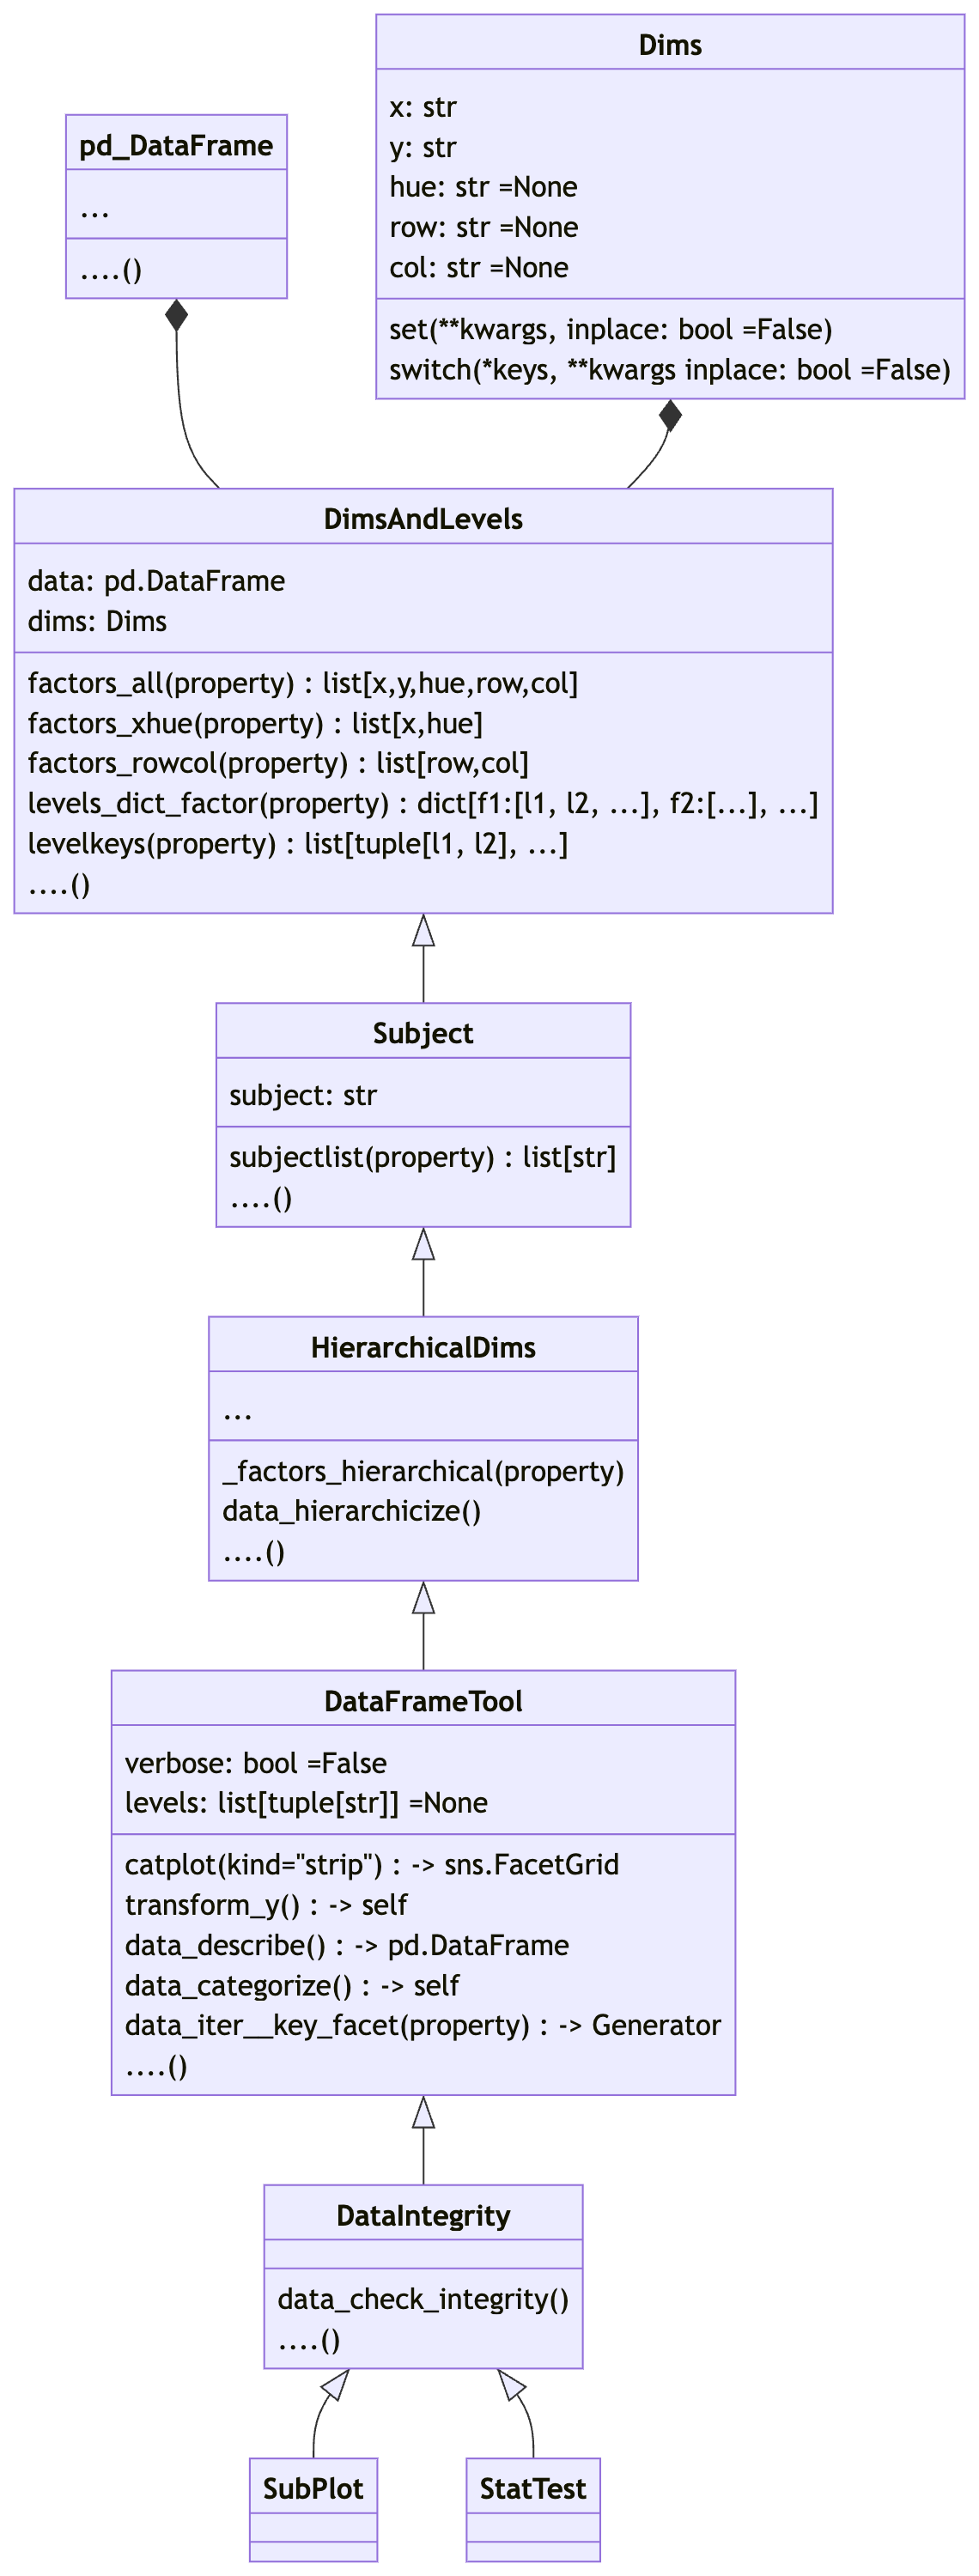
\includegraphics[scale=.18]{APPENDIX/classdiagr_dataframe.png}
    \caption{\mycap}
    \label{fig:classdiagr}
\end{figure}
\newpage

\setcounter{figure}{0} % > Reset figure counter
% > Lower part of Diagram
\def\mycap{\textbf{(continued)} The architecture of \texttt{plotastic}
    continues after the class \texttt{DataIntegrity} with classes for plotting
    (\texttt{SubPlot}) and statistical testing (\texttt{StatTest}) and end with
    the class \texttt{DataAnalysis}, which serves as the main user interface.
    \umlconvention }
\begin{figure}[H]
    \centering
    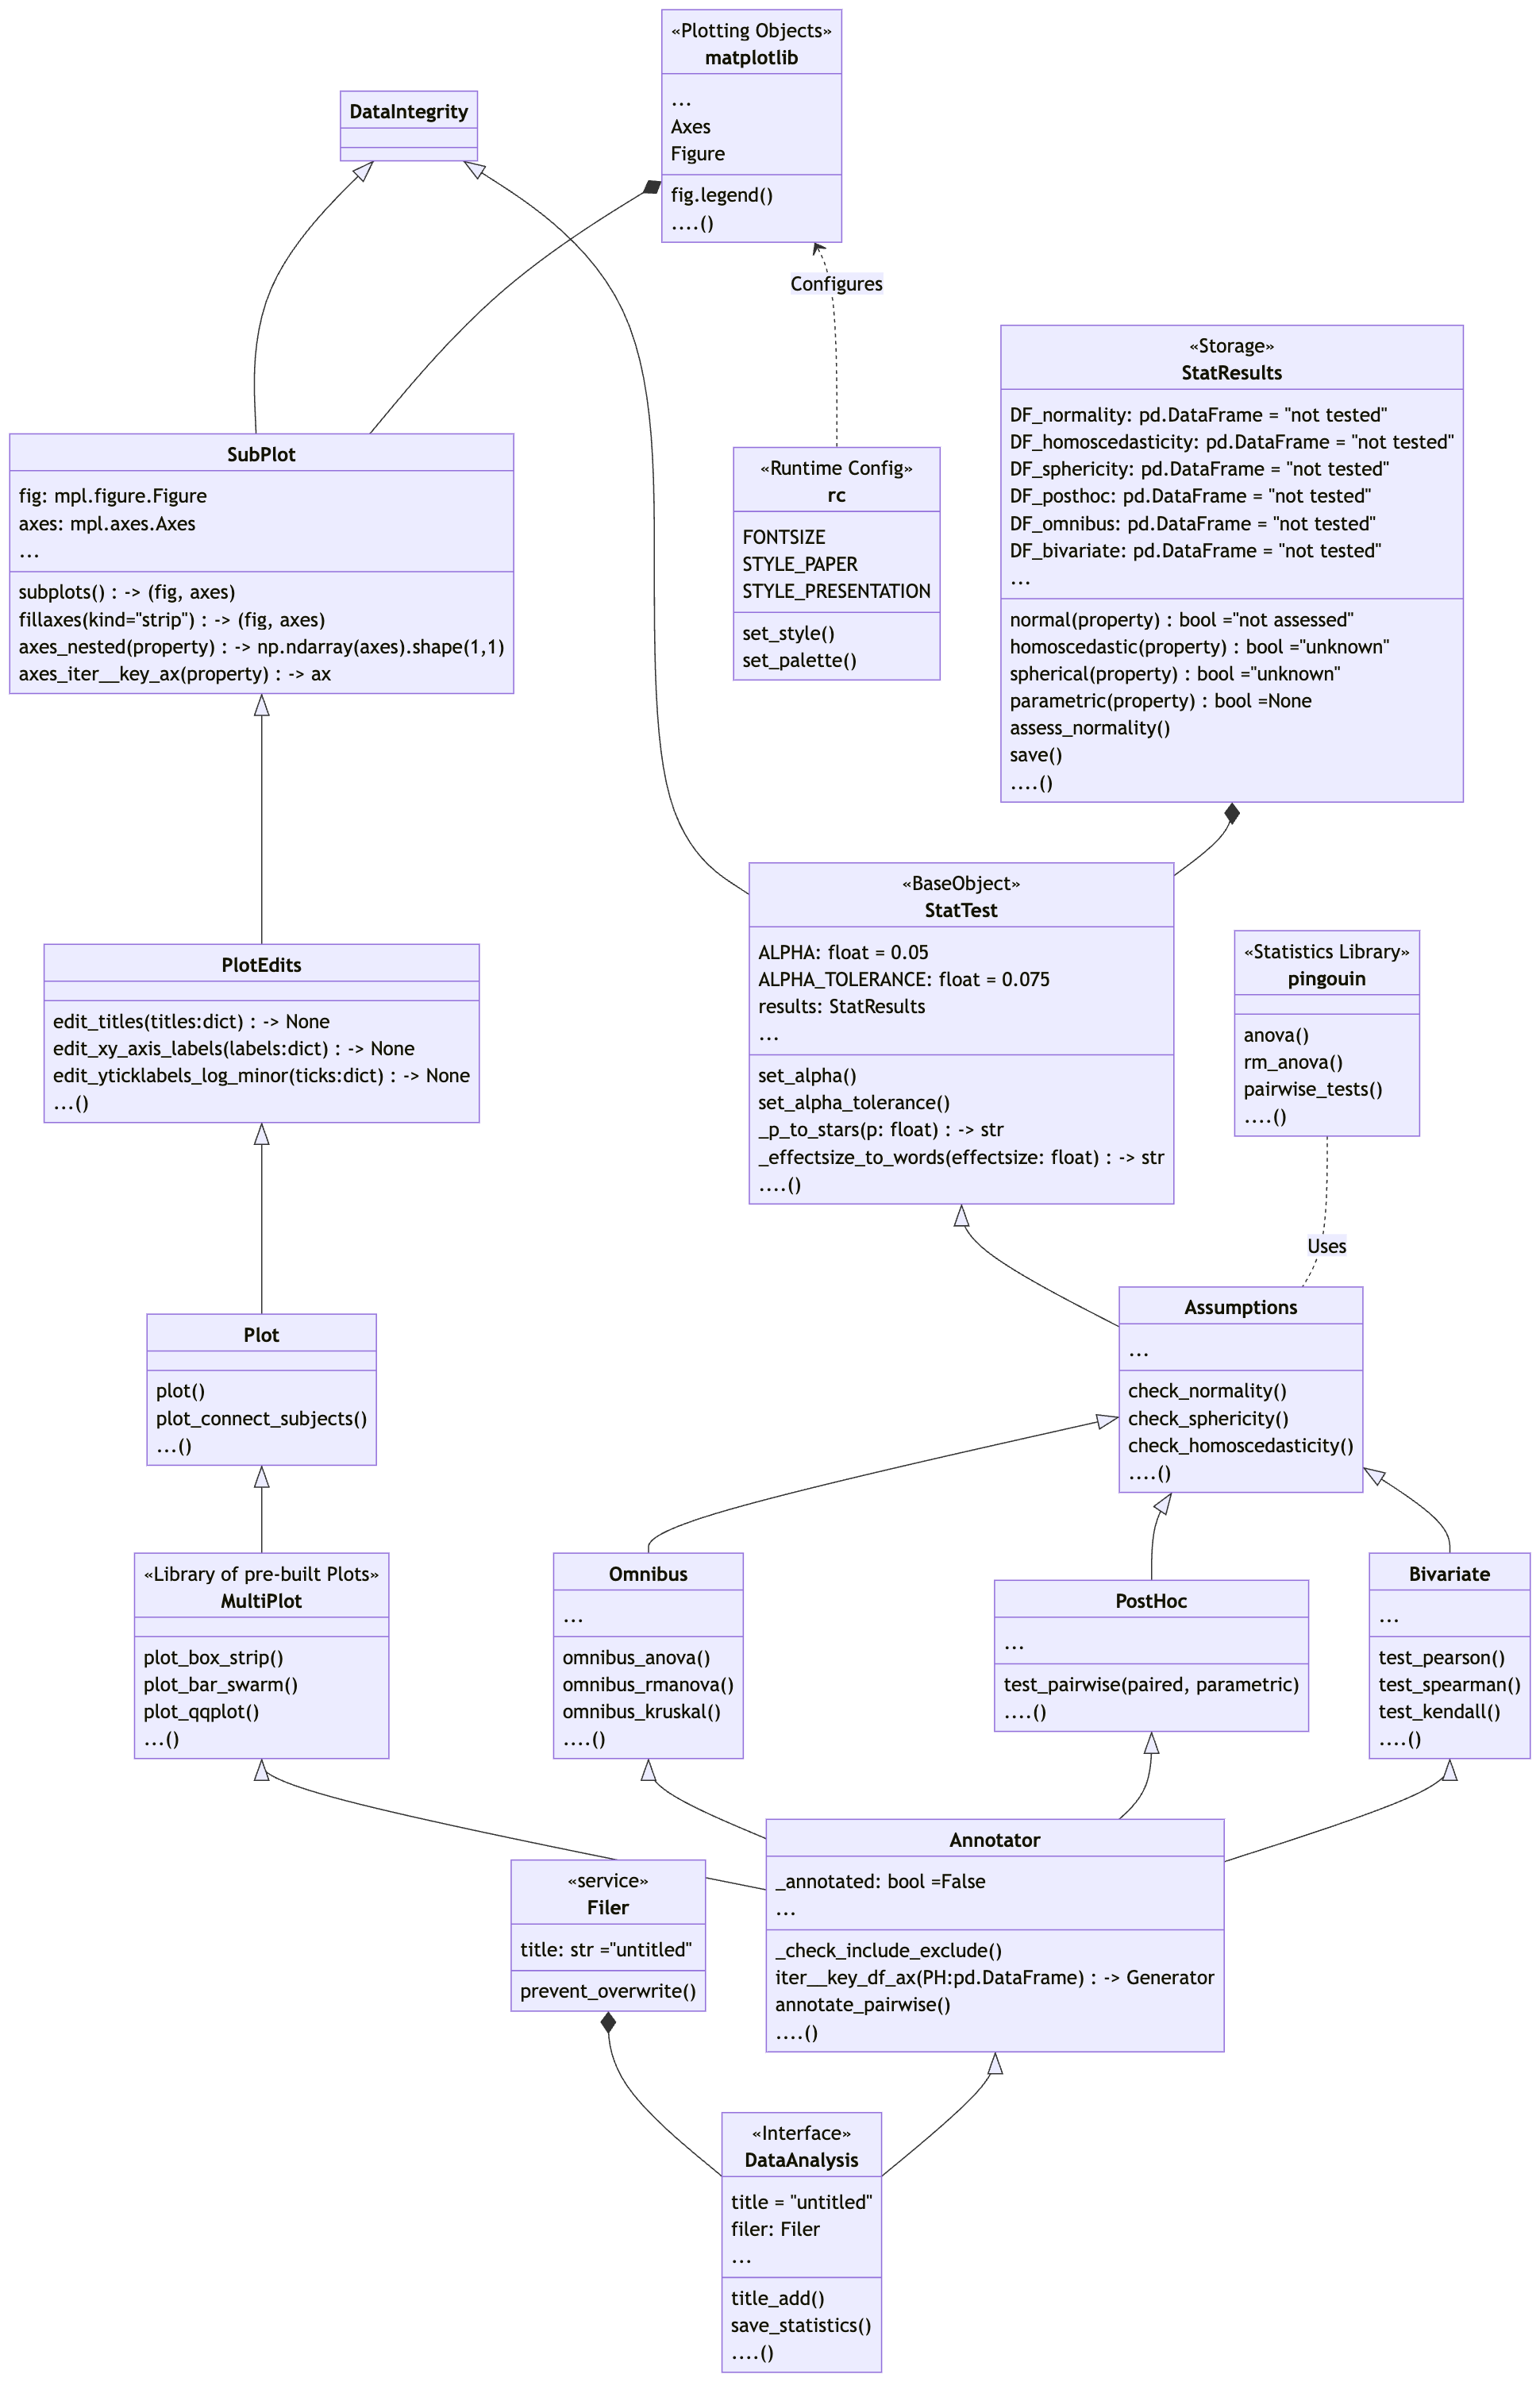
\includegraphics[scale=.20]{APPENDIX/classdiagr_plot+stats.png}
    \caption{\mycap}
\end{figure}



% == Readme from plotastic (PyPi) ======================================
% > Make an empty page with the section title
\def\mytitle{Readme of \texttt{plotastic}}
\markboth{Appendix}{: \mytitle}
\subsection*{\mytitle}
\ %
The following pages are the \texttt{README.md} of \texttt{plotastic} found in
the Python Package Index (PyPi) (\url{pypi.org/project/plotastic}), and on
GitHub (\url{github.com/markur4/plotastic}).

\addpdf[.93]{\mytitle}{APPENDIX/README_pypi.pdf}
\newpage




% == Example Analyses plotastic =======================================



% ======================================================================
% == CV 
% ======================================================================
\addpdfsection{Curriculum Vitae}{APPENDIX/CV Martin Kuric (eng).pdf}

\newpage

% ======================================================================
% == Affidavit / Eidestattliche Erklärung 
% ======================================================================
% \unnsection{Affidavit}
% \markboth{Affidavit}{}
\addpdfsection{Affidavit}{APPENDIX/Affidavit.pdf}






% ============
\end{document}
% ============